
%\documentclass[14pt]{extarticle}
\documentclass[12pt,a4paper]{scrbook}
\usepackage[cm-default]{fontspec}
\usepackage{csquotes}
\usepackage{url}
\usepackage[shortcuts]{extdash}
\usepackage{pgffor}
\usepackage[unicode=true]{hyperref}
%\usepackage{breakurl}
\usepackage{array}
%\usepackage{graphicx}
\usepackage[export]{adjustbox}
\usepackage{listings}
\renewcommand{\lstlistingname}{\inputencoding{latin0}Listing}

\usepackage{xcolor}

\usepackage{polyglossia,xunicode}
\setdefaultlanguage{english}
\setotherlanguage{tamil}
\setotherlanguage{portuguese}

\usepackage[normalem]{ulem}
%\usepackage[noend,noeledsec,noledgroup]{reledmac}
\renewcommand{\multfootsep}{\,}
\usepackage[margin=1in]{geometry}

\usepackage{footnote}
\makesavenoteenv{tabular}

\usepackage{setspace}
\onehalfspacing

\graphicspath{ {./assets/} {./img/} }

\usepackage{changepage}

\setlength{\parskip}{\medskipamount}
\setlength{\parindent}{0pt}

\setmainlanguage{english}
\setotherlanguage{tamil}
\setmainfont[
    Path = ./fonts/brill-typeface/,
    UprightFont = brill-roman,
    BoldFont = brill-bold,
    ItalicFont = brill-italic,
    BoldItalicFont = brill-bold-italic,
    Extension = .ttf]{Brill}
\newfontfamily{\defaultfont}[
    Path = ./fonts/brill-typeface/,
    UprightFont = brill-roman,
    BoldFont = brill-bold,
    ItalicFont = brill-italic,
    BoldItalicFont = brill-bold-italic,
    Extension = .ttf]{Brill}
\newfontfamily{\tamilfont}[
    Path = ./fonts/,
    UprightFont = ArimaMadurai-Light,
    BoldFont = ArimaMadurai-Medium,
    Extension = .ttf]{ArimaMadurai}

\usepackage[Tamil,Latin]{ucharclasses}
\setDefaultTransitions{\defaultfont}{}
\setTransitionsForLatin{\defaultfont}{}
\setTransitionTo{Tamil}{\tamilfont}

%\usepackage[style=chicago-authordate,natbib=true,backend=biber,maxcitenames=2]{biblatex}
%\usepackage{cite}

\begin{document}
    \begin{titlepage}

    \title{\emph{Tamil grammar in Portugese}}\subtitle{A diplomatic edition of Indien 188c, Bibliothèque nationale de France}\author{Cristina MURU}
\date{}
\publishers{
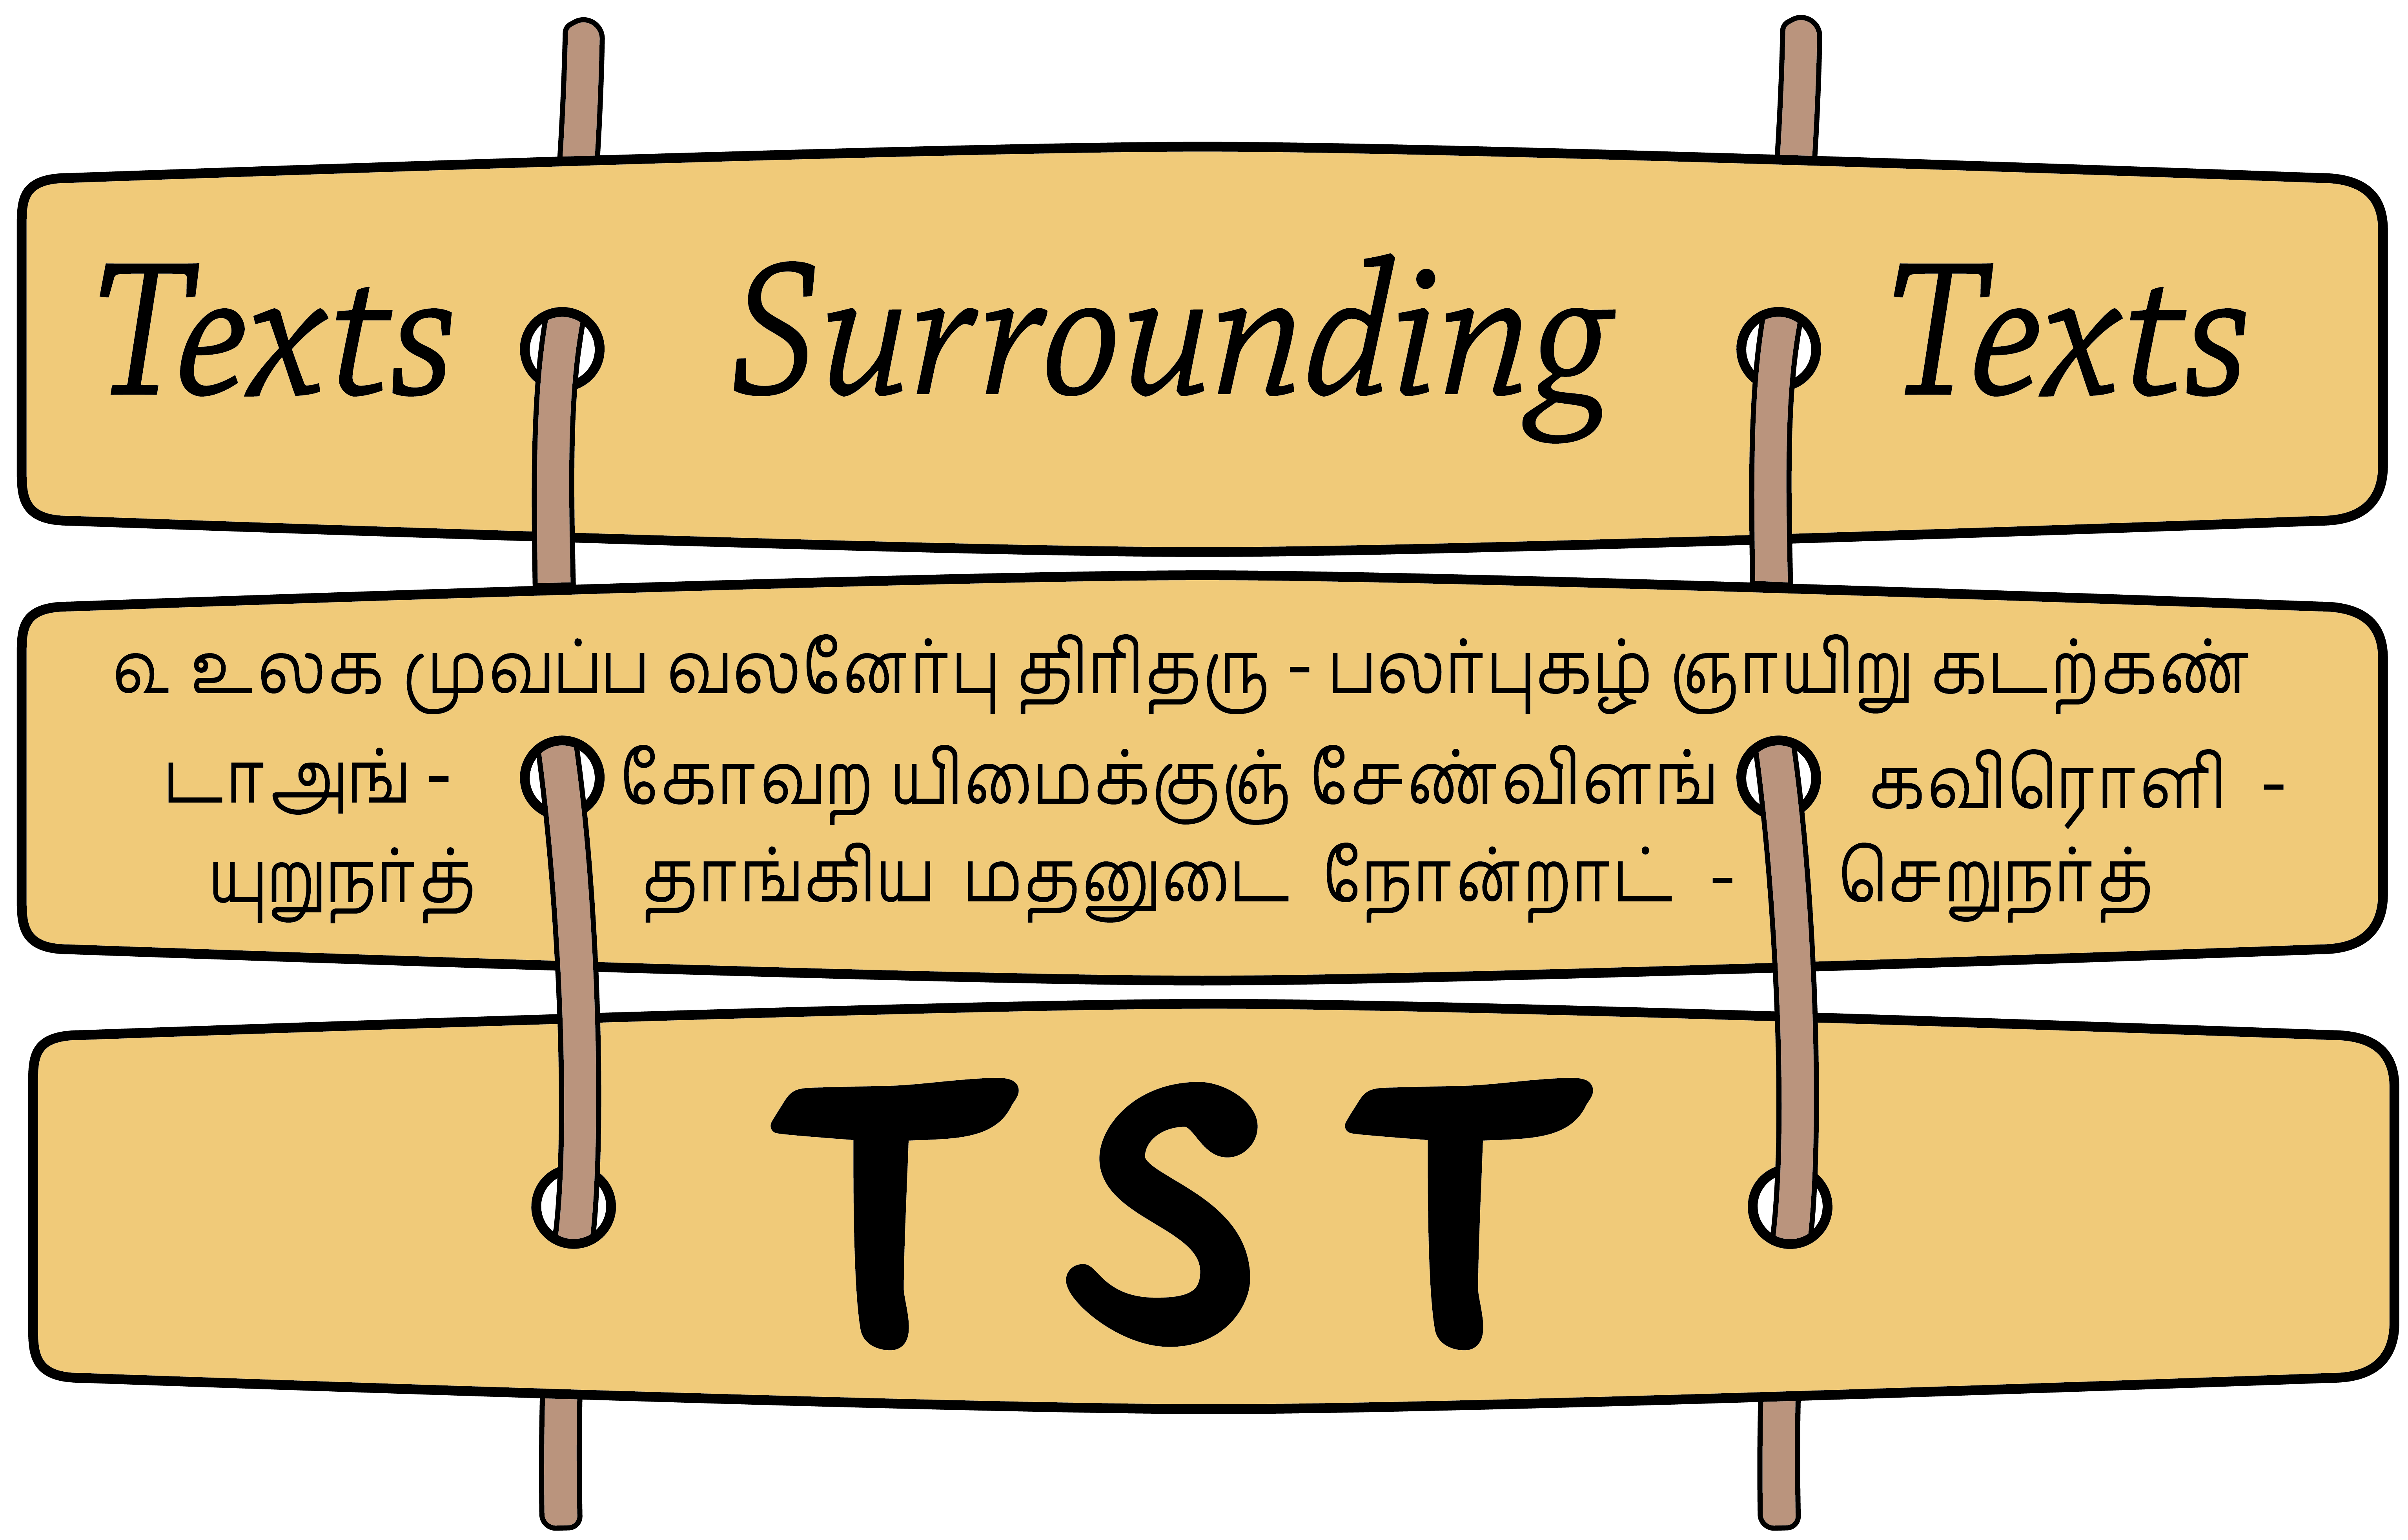
\includegraphics[height=2em]{tst}\\
Texts Surrounding Texts\\
Paris · Hamburg
}   
\end{titlepage}
    
\lowertitleback{
    
\includegraphics[height=1em]{cc.xlarge} 
\includegraphics[height=1em]{by.xlarge} 
\includegraphics[height=1em]{nc-eu.xlarge} 2022 Cristina MURU\\
    This text is licensed under a Creative Commons Attribution-NonCommercial license.\\
    Manuscript images are courtesy of Gallica / Bibliothèque nationale de France.\\
    \\
    ISBN XXXX-XXXX-XXXX eBook\\
    \\
    Text Surrounding Texts (FRAL 2018, ANR/DFG)\\
    Centre nationale de la recherche scientifique\\
    Paris, France\\
    \\
    
\includegraphics[height=2em]{anr} \hfill 
\includegraphics[height=2em]{bnf} \hfill 
\includegraphics[height=1.8em]{dfg} \\
}
    \maketitle
    \newpage
    \begin{center}\textsc{TST Diplomatic Editions}\\

    \quotation{This edition has been published as part of the Texts Surrounding Texts project, funded jointly by the Agence nationale de la recherche in France and the Deutsche Forschungsgemeinschaft in Germany. TST Diplomatic Editions publishes unique and important manuscripts from the collection of the Bibliothèque nationale de France.}
    \end{center}
    
\newpage

\tableofcontents

\part{Introduction}
    
\part{The manuscript}
\newpage
    
              

A grammar of Tamil language in Portuguese, containing descriptions and explanations about declensions, conjugation and syntax.
                     
\begin{itemize}
    
\item First come the declensions (\hyperlink{img-25}{f8r}‒\hyperlink{img-35}{f13r}). The nouns chosen for illustrating the declensions are the same as those found in \emph{Arte da lingua Malabar} composed around 1549 by the Jesuit Henrique Henriques (1520‒1600). For instance, the first declension of Henriques corresponds to the sixth declension here; the third to the fourth; the fourth to the first; and the fifth to the third. The second declension is the same in both.
    
\item We find afterwards explanations about nouns and adjectives, e.g.: “os nomes acabados em ஆ â (…)” (\hyperlink{img-37}{f14r}); “dos Nomes adiectiuos” (\hyperlink{img-39}{f15r}); “dos Comparatiuos” (\hyperlink{img-41}{f16v}); “dos Superlatiuos” (\hyperlink{img-43}{f17r}); “dos nomens de qualidade et gantidade” (\hyperlink{img-44}{f17v}); “pera os nomens de quantidade” (\hyperlink{img-45}{f18r}\hyperlink{img-46}{v}) ; “dos nomens Numerais” (\hyperlink{img-47}{f19r}‒\hyperlink{img-51}{21r}) ; “dos pronomens” (\hyperlink{img-51}{f21r}).
    
\item Then comes the book II on verbs (“Livro 2° dos verbos,” (\hyperlink{img-57}{f24r}). The following headears are found in this portion of the text: “primeira Conjugacaõ” (\hyperlink{img-57}{f24r}); “2a Conjugacaõ” (\hyperlink{img-69}{f30r}); “3a Conjugacaõ” (\hyperlink{img-79}{f35r}); “4a Conjugacaõ” (\hyperlink{img-83}{f37r}); “5a Conjugacaõ” (\hyperlink{img-87}{f39r}); “dos uerbos Compositos” (\hyperlink{img-91}{f41r}); “dos uerbos passiuos” (\hyperlink{img-91}{f41v}); “Dos uerbos Impersoaes” (\hyperlink{img-93}{f42r}); “dos uerbos defeitivos”” (\hyperlink{img-96}{f43v}).
    
\item Finally from \hyperlink{img-100}{f45v}, various topics are discussed, e.g.: “dos partecipios” (\hyperlink{img-100}{f45v}); “do casu” (\hyperlink{img-100}{f45v}); “do Dativo” (\hyperlink{img-102}{f46v}); “por Accusativo” (\hyperlink{img-103}{f47r}); “por ablatiuo” (\hyperlink{img-104}{f47v}); “dos partecipios adiectiuos” (\hyperlink{img-108}{f49v}); “dos partecipios do Infinito” (\hyperlink{img-108}{f49v}); “dos tempos menos principaes” (\hyperlink{img-109}{f50r}); “da particula, Am” (\hyperlink{img-114}{f52v}); “das proposicoens” (\hyperlink{img-116}{f53v}); “aduerbios de tempo” (\hyperlink{img-118}{f54v}); “de responder” (\hyperlink{img-119}{f55r}); “de afirmar” (\hyperlink{img-119}{f55r}); “de negar” (\hyperlink{img-119}{f55r}); “de quandidade” (\hyperlink{img-121}{f56r}); “modo de formar os uerbos” (\hyperlink{img-122}{f56v}).
    
\item The last folio is about “de quantitade” (\hyperlink{img-121}{f56r}). The \hyperlink{img-123}{f57v} bears a crossed-out word.
    
\end{itemize}
    
                    
            
\cleardoublepage
\makeatletter\@openrightfalse
\part{Diplomatic edition}
    
    
      
\newpage
\hypertarget{img-25}{
    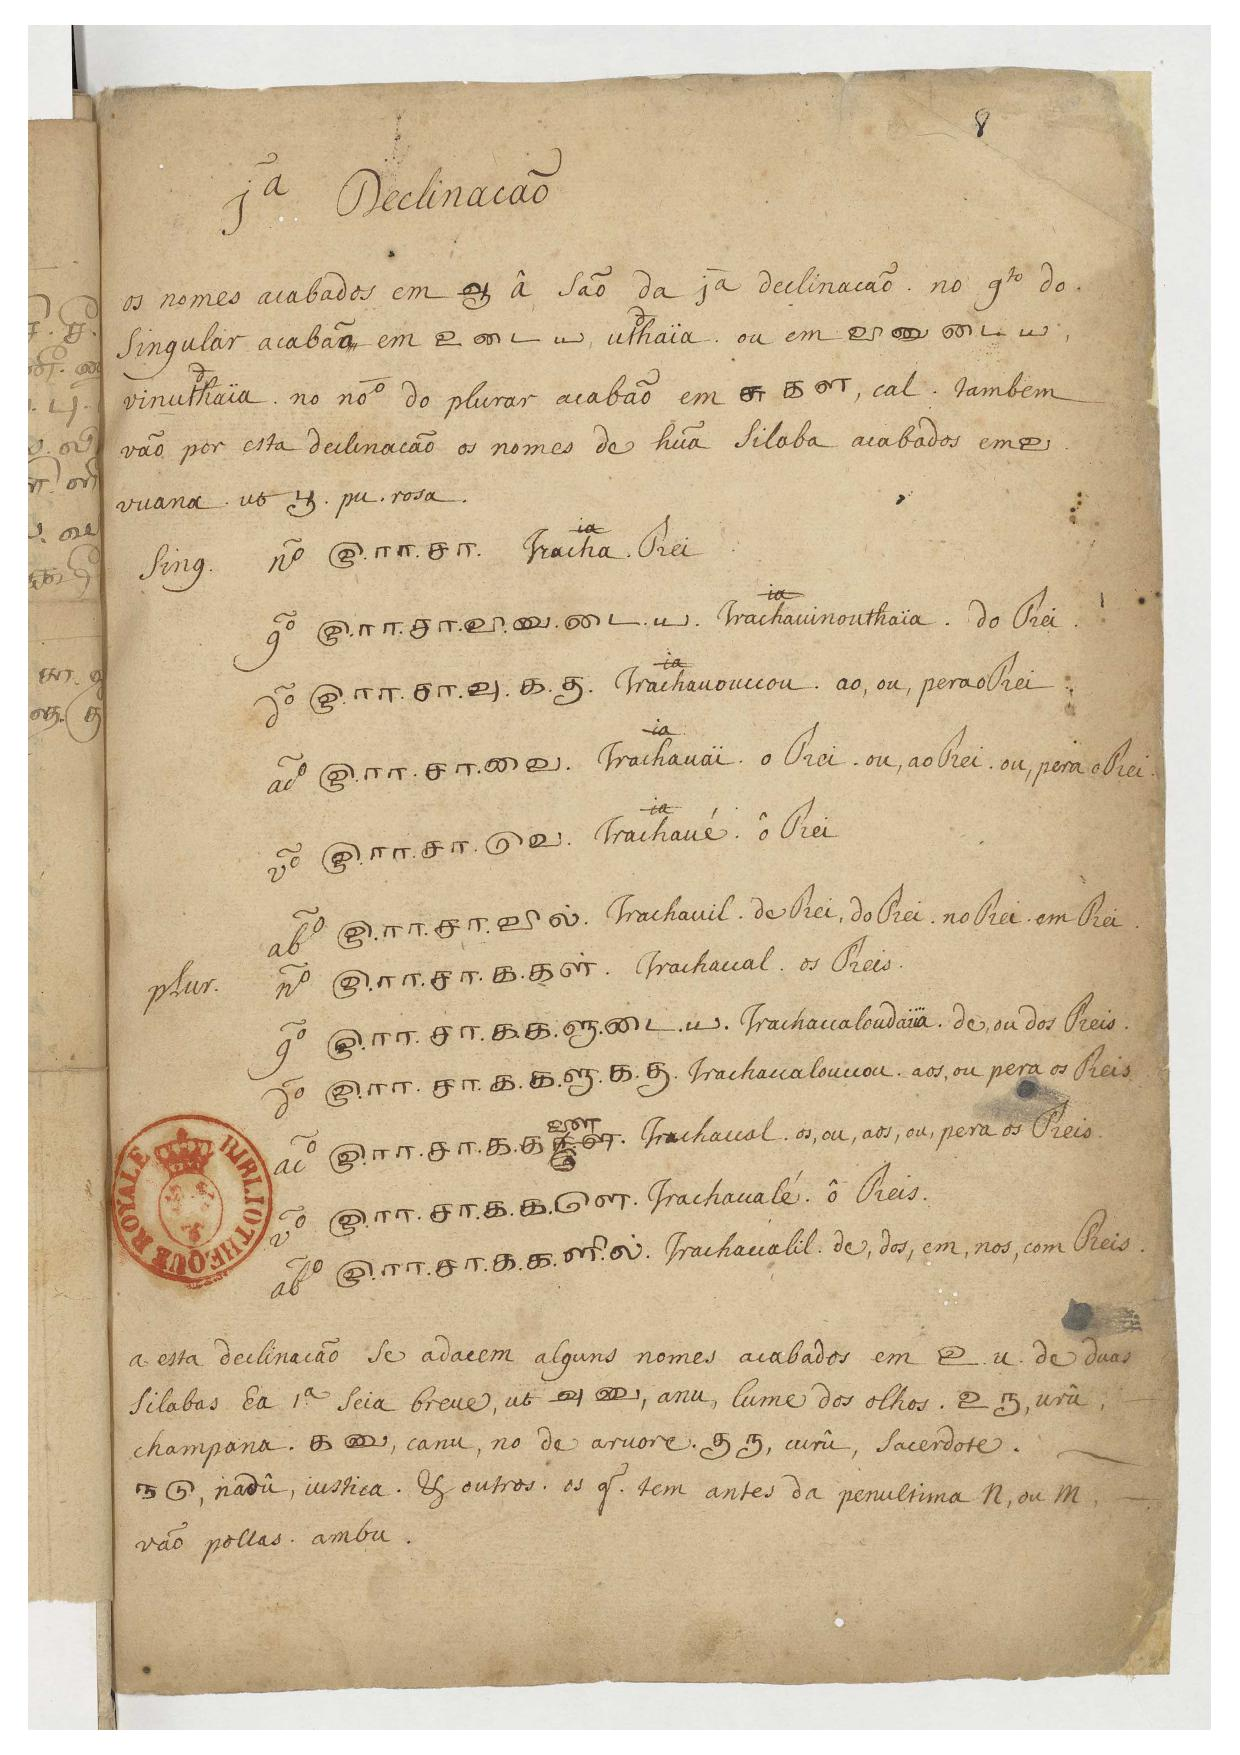
\includegraphics[width=\textwidth]{img-25}}
\newpage
      \chapter*{1ª Declinacaõ}
    \addcontentsline{toc}{chapter}{1ª Declinacaõ}
    
      

Os nomes acabados em ஆ â saõ da 1° declinaçaõ no g[enitiv]o do 
            singular acabaõ em உடைய uthaïa ou em வினுடய
            vinuthaïa no n[ominativ]o do plural acabaõ em ககள, cal . Tambem
            vaõ por esta declinacaõ os nomes e huã silaba acabados em வ
            vuana ut பூ pu.rosa. 
        
      
\begin{tabular}{lllll}
    
        
          Sing. &
          n\textsuperscript{õ} &
          இ.ரா.சா. &
          iracha &
          Rei \\
    
        
    
        
           &
          g\textsuperscript{õ} &
          இ.ரா.சா.வினு.டை.ய &
          irachavinouthaïa &
          do Rei \\
    
        
    
        
           &
          d\textsuperscript{õ} &
          இ.ரா.சா.வு.ககு &
          irachavouccou &
          au, ou, pera o Rei \\
    
        
    
        
           &
          ac\textsuperscript{õ} &
          இ.ரா.சா.வை &
          irachavaï &
          o Rei, ou, ao Rei, ou, pera o Rei \\
    
        
    
        
           &
          v\textsuperscript{õ} &
          இ.ரா.சா.வெ &
          irachavé &
          ô Rei \\
    
        
    
        
           &
          ab\textsuperscript{õ} &
          இ.ரா.சா.வில &
          irachavil  &
          de Rei, do Rei, no Rei, em Rei \\
    
        
    
        
          plur. &
          n\textsuperscript{õ} &
          இ.ரா.சா.ககள &
          irachaccal &
          os Reis \\
    
        
    
        
           &
          g\textsuperscript{õ} &
          இ.ரா.சா.க்களு.டை.ய &
          irachaccaloudaïa  &
          de ou dos Reis \\
    
        
    
        
           &
          d\textsuperscript{õ} &
          இ.ரா.சா.க.க.ளு.க.கு &
          irachaccalouccou &
          aos, ou pera os Reis \\
    
        
    
        
           &
          ac\textsuperscript{õ}\footnote{At the beginning the scribe writes iracchacaḷ, then he corrects it in -cale, and finally in -caḷai.} &
          இ.ரா.சா.க.க.ளை &
          irachaccal &
          os, ou, aos, ou, pera os Reis \\
    
        
    
        
           &
          v\textsuperscript{õ} &
          இ.ரா.சா.க.க.ளெ &
          irachaccalé &
          ô Reis \\
    
        
    
        
           &
          ab\textsuperscript{õ} &
          இ.ரா.சா.க.க.ளில் &
          irachaccalil  &
          de, dos, em, nos, com Reis \\
    
        
    
      
\end{tabular}
    
      

a esta declinacaõ se adacem alguns nomes acabados em உ u de doas silabas e a 1° seia breve, ut அனு, anu, lume dos olhos, உரு, urû, champana, கனு, canu, no de arvore. குரு, curû, sacerdote. நடு, nadû, iustica. Et outros os q[uaes] tem antes da penultima n, ou m, vaõ pollas amba.
      
\newpage
\hypertarget{img-27}{
    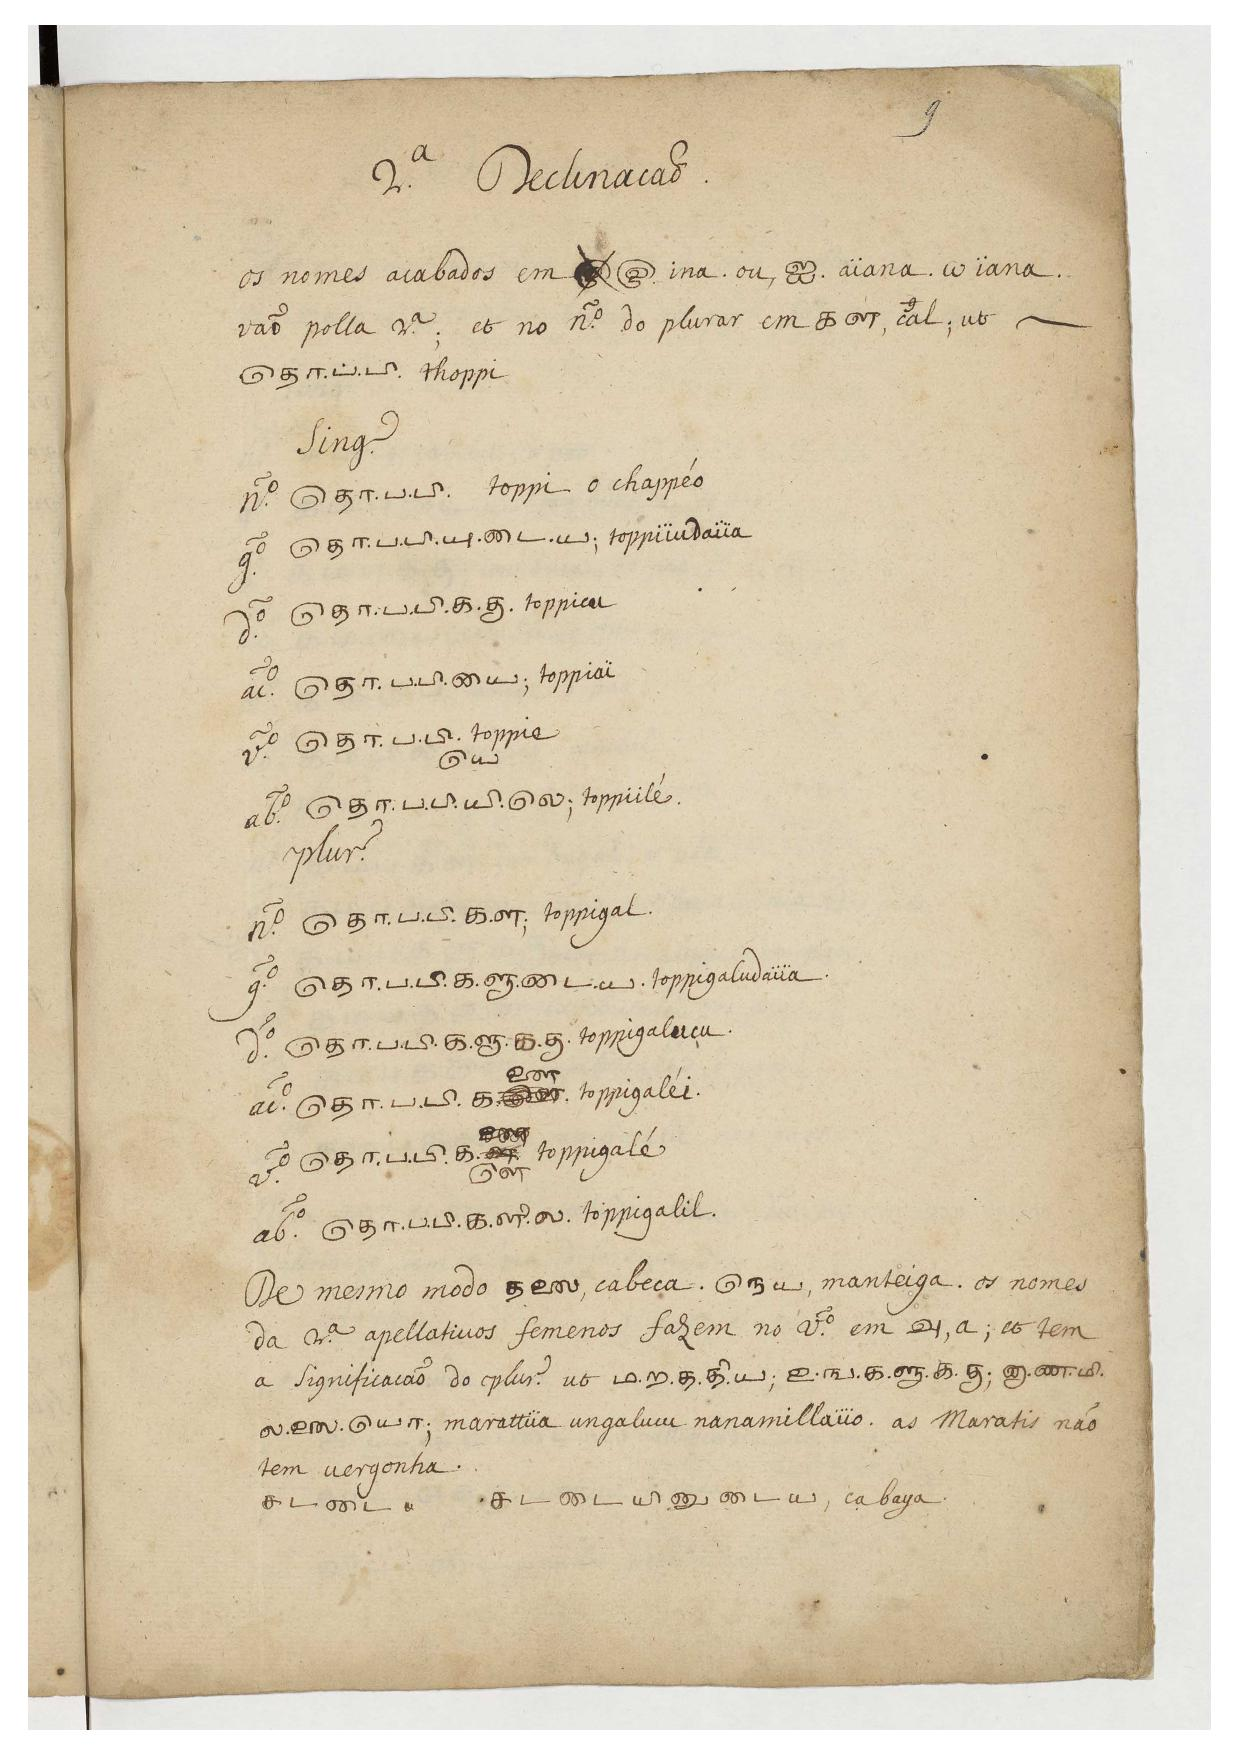
\includegraphics[width=\textwidth]{img-27}}
\newpage
      \chapter*{2ª Declinacaõ}
    \addcontentsline{toc}{chapter}{2ª Declinacaõ}
    
      

os nomes acabados em \sout{\textcolor{gray}{இ}}இ ina, ou ஐ, aïana, ய, ïana 
            vaõ polla 2° et no n[ominativ]o do plurar em கள cal, 
            ut தொ.ப்.பி thoppi.
        
      
\begin{tabular}{lllll}
    
        
          Sing. &
          n\textsuperscript{õ} &
          தொ.ப.பி &
          toppi &
          o chappéo \\
    
        
    
        
           &
          g\textsuperscript{õ} &
          தொ.ப.பி.யு.டை.ய &
          toppïïudaïa &
           \\
    
        
    
        
           &
          d\textsuperscript{õ} &
          தொ.ப.பி.க.கு &
          toppicu &
           \\
    
        
    
        
           &
          ac\textsuperscript{õ} &
          தொ.ப.பி.யை &
          toppiaï &
           \\
    
        
    
        
           &
          v\textsuperscript{õ} &
          தொ.ப.பி.யெ &
          toppia &
           \\
    
        
    
        
           &
          ab\textsuperscript{õ} &
          தொ.ப.பி.யி.லெ &
          toppiilé &
           \\
    
        
    
        
          plur. &
          n\textsuperscript{õ} &
          தொ.ப.பி.க.ள &
          toppigal &
           \\
    
        
    
        
           &
          g\textsuperscript{õ} &
          தொ.ப.பி.க.ளு.டை.ய &
          toppigaludaïïa &
           \\
    
        
    
        
           &
          d\textsuperscript{õ} &
          தொ.ப.பி.க.ளு.க.கு &
          toppigalucu &
           \\
    
        
    
        
           &
          ac\textsuperscript{õ} &
          தொ.ப.பி.க.\sout{\textcolor{gray}{ளெ}}\textbf{ளை} &
          toppigaléi &
           \\
    
        
    
        
           &
          v\textsuperscript{õ} &
          தொ.ப.பி.க.\sout{\textcolor{gray}{ள}}\sout{\textcolor{gray}{\textbf{ளை}}}\textbf{ளெ} &
          toppigalé &
           \\
    
        
    
        
           &
          ab\textsuperscript{õ} &
          தொ.ப.பி.க.ளி.ல &
          toppigalil &
           \\
    
        
    
      
\end{tabular}
    
      

de mesmo modo தலை cabeca. நெய manteiga. Os nomes 
            da 2ª appellativos femenos fazem no v[ocativ]o em அ, a; et tem
            a significacaõ do plural ut ம.ற.த.தி.ய, உ.ங.க.ளு.க.கு, னா.ண.மி.
            ல.லை.யொ; marattïa ungaluccu nanamillaïïo, as Maratis naõ tem vergonha.
        
      

சடடைசடடையினுடைய cabaya
        
      
\newpage
\hypertarget{img-29}{
    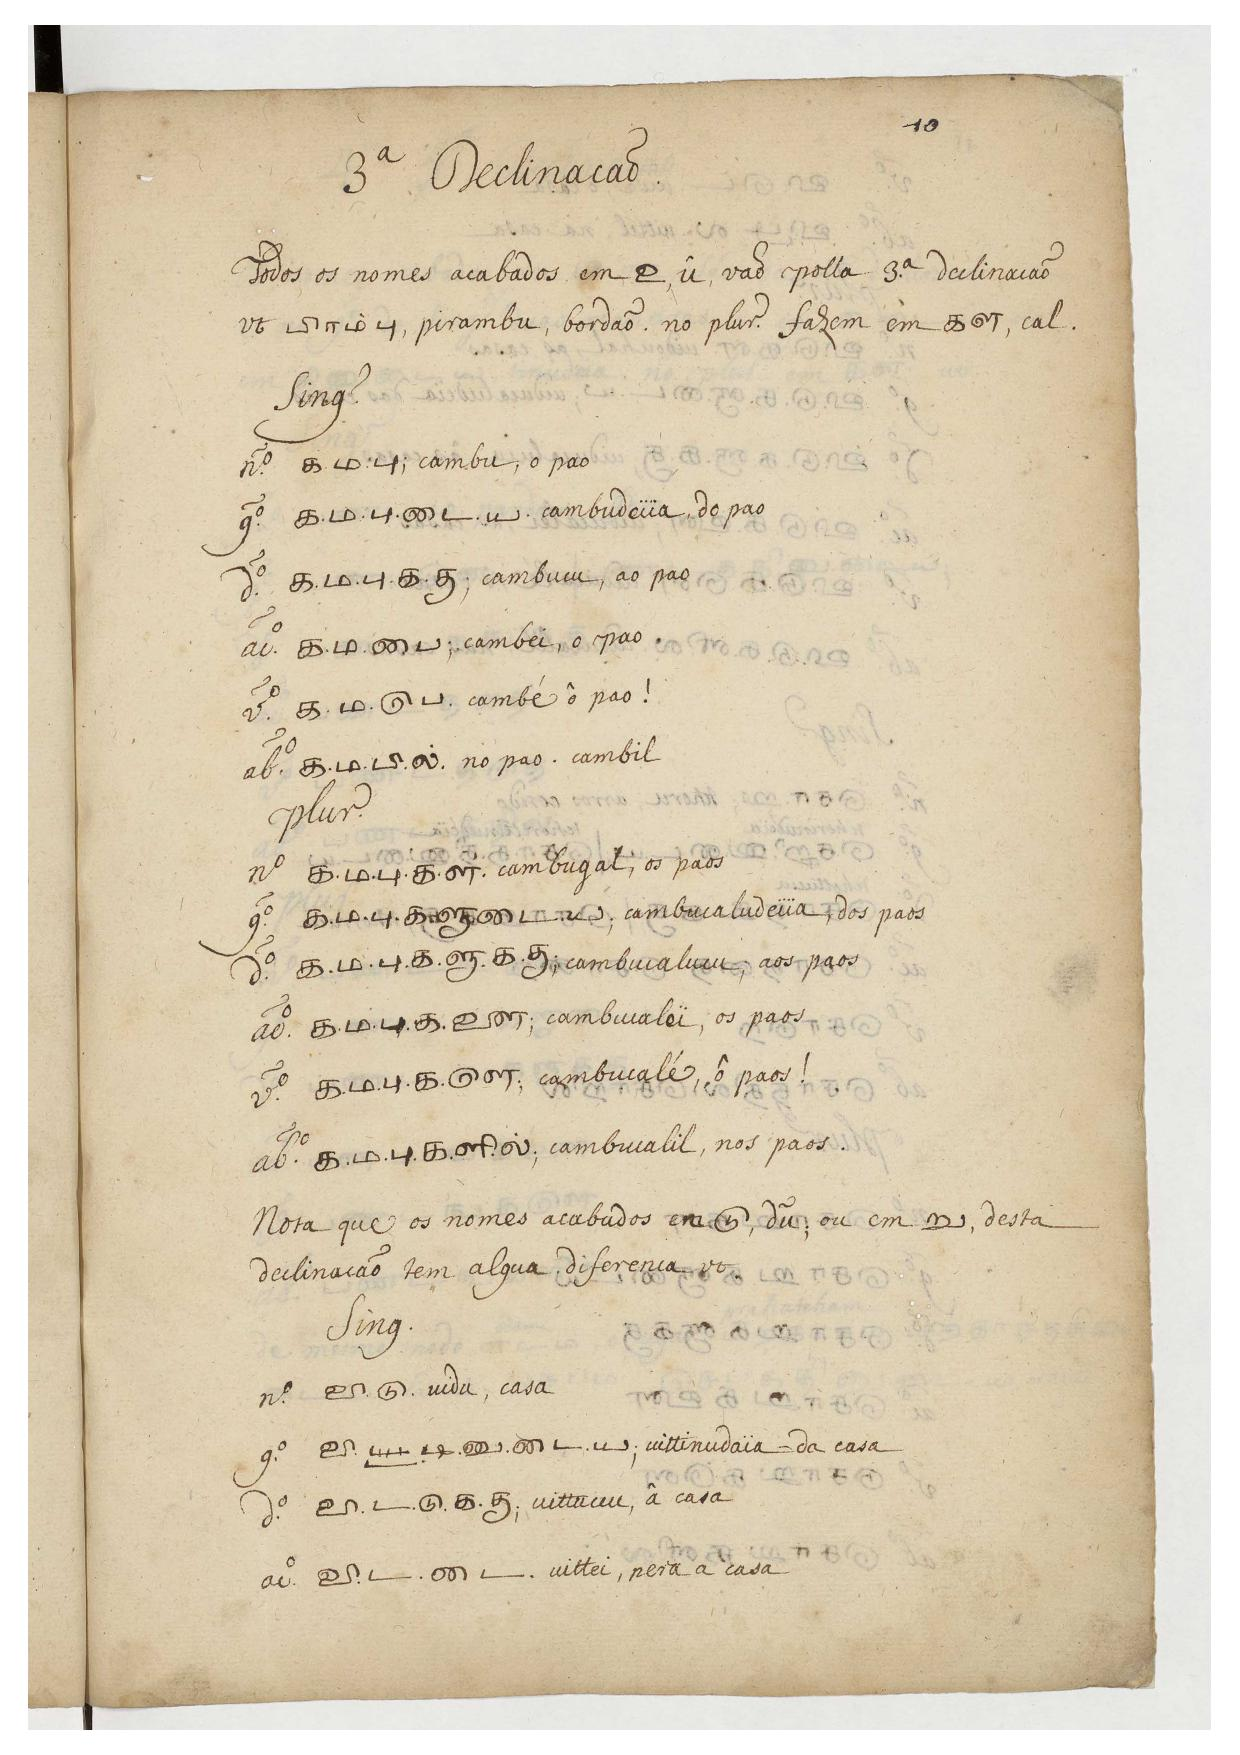
\includegraphics[width=\textwidth]{img-29}}
\newpage
      \chapter*{3ª Declinacaõ}
    \addcontentsline{toc}{chapter}{3ª Declinacaõ}
    
      

 Todos os nomes acabados em உ û,vaõ polla 3ª declinação 
             ut பிரம்பு, pirambu bordaõ no plural fazem em கள, cal.
        
      
\begin{tabular}{lllll}
    
        
          Sing. &
          n\textsuperscript{õ} &
          கம.பு &
          cambu &
          o pao \\
    
        
    
        
           &
          g\textsuperscript{õ} &
           க.ம.பு.டை.ய &
          cambudeïïa &
          do pao \\
    
        
    
        
           &
          d\textsuperscript{õ} &
          க.ம.பு.க.கு &
          cambucu &
          ao pao \\
    
        
    
        
           &
          ac\textsuperscript{õ} &
          க.ம.பை &
          cambei &
          o pao \\
    
        
    
        
           &
          v\textsuperscript{õ} &
          க.ம.பெ &
          cambé &
          ô pao! \\
    
        
    
        
           &
          ab\textsuperscript{õ} &
          க.ம.பி.ல் &
          no pao &
          cambil \\
    
        
    
        
          plur. &
          n\textsuperscript{õ} &
          க.ம.பு.க.ள &
          cambugal &
          os paos \\
    
        
    
        
           &
          g\textsuperscript{õ} &
          க.ம.பு.க.ளு.டை.ய &
          cambudeïïa &
          dos paos \\
    
        
    
        
           &
          d\textsuperscript{õ} &
          க.ம.பு.க.ளு.க.கு &
          cambucalucu &
          aos paos \\
    
        
    
        
           &
          ac\textsuperscript{õ} &
          க.ம.பு.க.ளை &
          cambucalaï &
          os paos \\
    
        
    
        
           &
          v\textsuperscript{õ} &
          க.ம.பு.க.ளெ &
           cambucalé &
          ô paos! \\
    
        
    
        
           &
          ab\textsuperscript{õ} &
          க.ம.பு.க.ளி.ல &
          cambucalil &
          nos paos \\
    
        
    
      
\end{tabular}
    
      

nota que os nomes acabados em டுdũ ou em று desta declinacaõ tem algua diferenca vt:
        
        
\begin{tabular}{lllll}
    
          
            Sing. &
            n\textsuperscript{õ} &
            விடு &
            vidu &
            casa \\
    
          
    
          
             &
            g\textsuperscript{õ} &
             விடடி.னு.டை.ய &
            vittinudaïa &
            da casa \\
    
          
    
          
             &
            d\textsuperscript{õ} &
             வி.டடு.க.கு &
            vittuccu &
            â casa \\
    
          
    
          
             &
            ac\textsuperscript{õ} &
            விடடை &
            vittei &
            pera a casa \\
    
          
    
          
\end{tabular}
    
          
\newpage
\hypertarget{img-31}{
    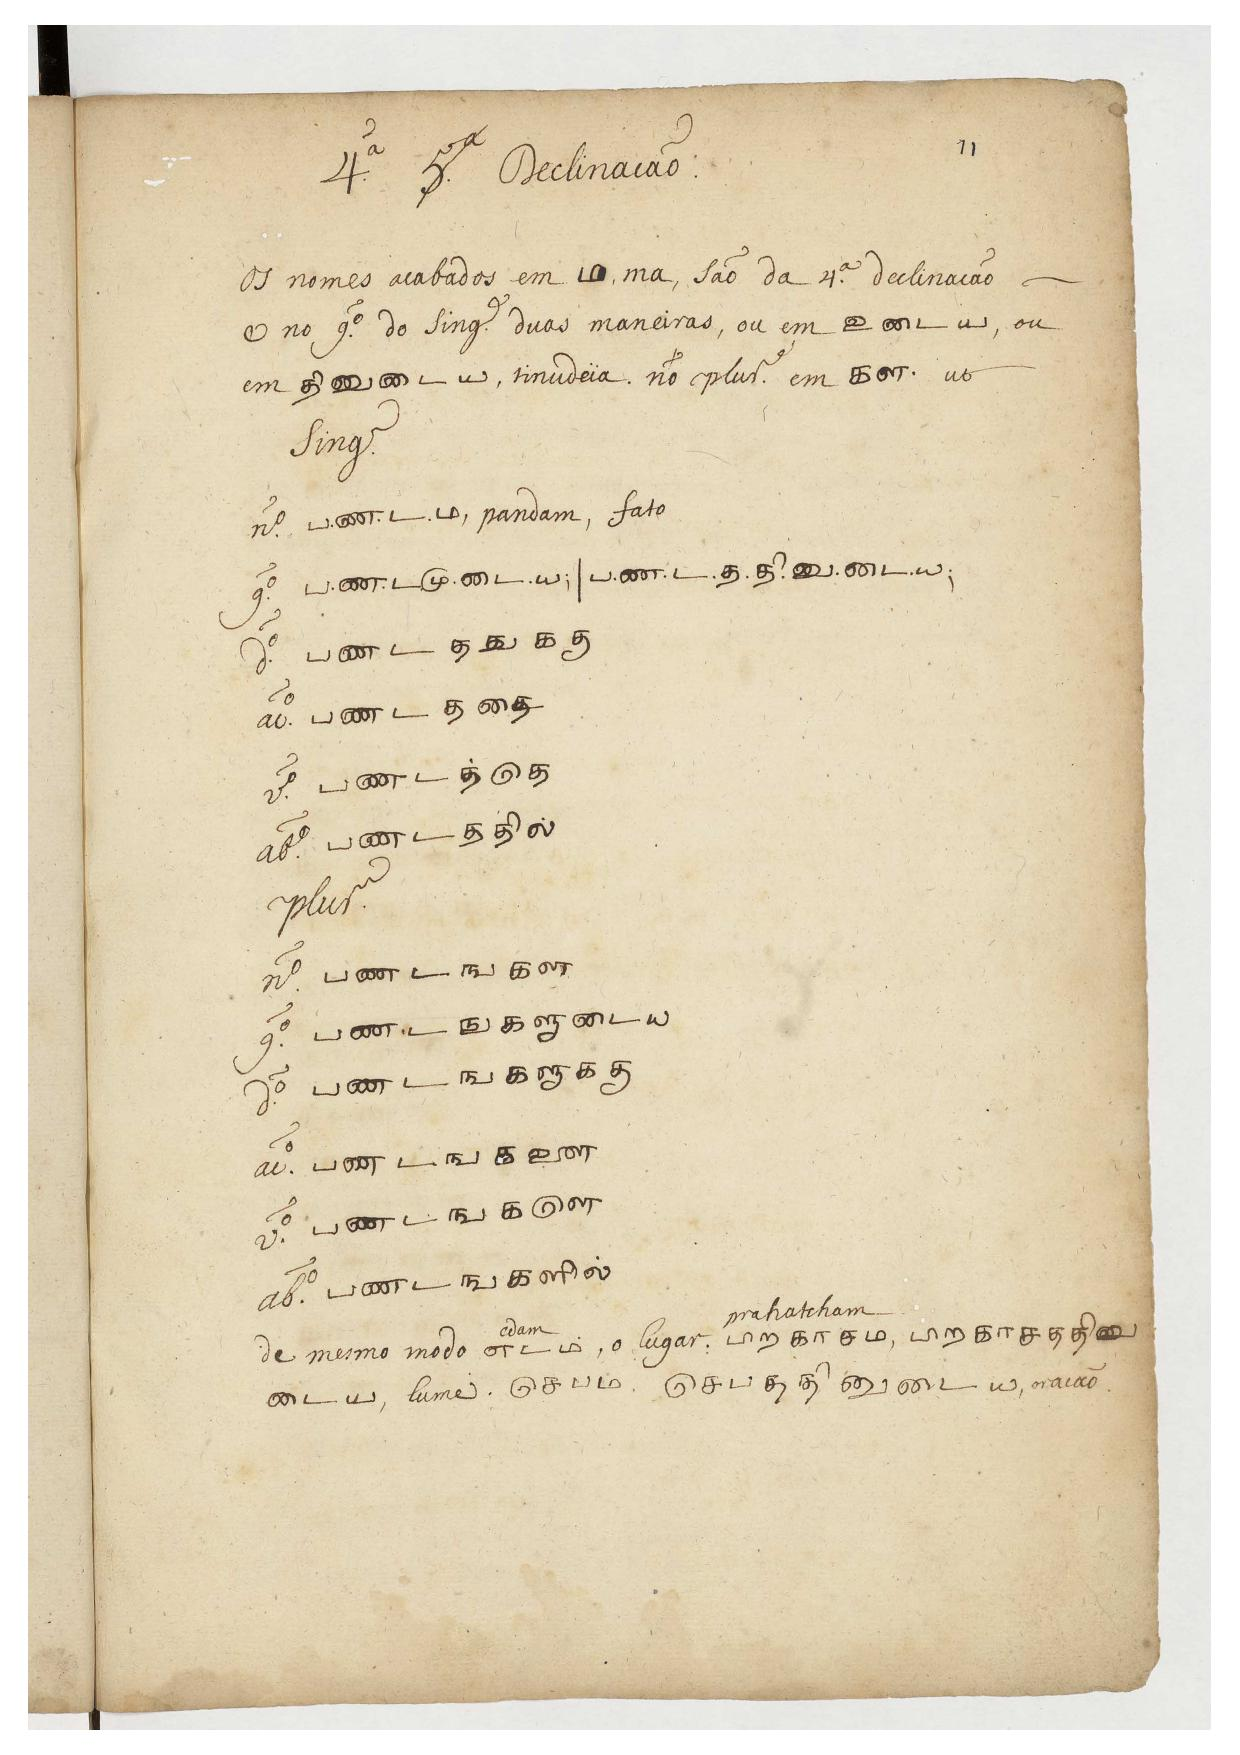
\includegraphics[width=\textwidth]{img-31}}
\newpage
          
\begin{tabular}{lllll}
    
          
             &
            v\textsuperscript{õ} &
            விடெ &
            vidé &
            ô casa \\
    
          
    
          
             &
            ab\textsuperscript{õ} &
            வி.டடி.ல &
            na casa &
            vittil \\
    
          
    
          
            plur. &
            n\textsuperscript{õ} &
            விடு.க.ள &
            vidouhal &
            as casas \\
    
          
    
          
             &
            g\textsuperscript{õ} &
            விடு.க.ளு.டை.ய &
             viducaludeïa &
            das casas \\
    
          
    
          
             &
            d\textsuperscript{õ} &
            விடு.க.ளு.க.கு &
            viducalucu &
            âs casas \\
    
          
    
          
             &
            ac\textsuperscript{õ} &
            விடு.க.ளை &
            viducalaï &
            as casas \\
    
          
    
          
             &
            v\textsuperscript{õ} &
            விடு.க.ளெ &
            viducalé &
            ô casas! \\
    
          
    
          
             &
            ab\textsuperscript{õ} &
            வி.டு.க.ளி.ல &
            viducalil &
            nas casas \\
    
          
    
          
            Sing. &
            n\textsuperscript{õ} &
            சொ.று &
            tchoru &
            arros cosido \\
    
          
    
          
             &
            g\textsuperscript{õ} &
             சொ.றி.னு.டை.ய &
             சொ.ததி.னு.டை.ய &
            tchorinudaïïa &
            tchorittinudèïa \\
    
          
    
          
             &
            d\textsuperscript{õ} &
            சொ.தது.க.கு &
             சொ.று.ககு &
            tchottuccu &
            tchorruccu \\
    
          
    
      
\end{tabular}
    
        
\begin{tabular}{llll}
    
          
             &
            ac\textsuperscript{õ} &
            சொ.ததை &
            சொ.றை \\
    
          
    
          
             &
            v\textsuperscript{õ} &
            சொ.றெ \\
    
          
    
          
             &
            ab\textsuperscript{õ} &
            சொததில் &
            சொறில \\
    
          
    
          
            plur. &
            n\textsuperscript{õ} &
            சொறுகள \\
    
          
    
          
             &
            g\textsuperscript{õ} &
            சொறுகளுடைய \\
    
          
    
          
             &
            d\textsuperscript{õ} &
            சொறுகளுககு \\
    
          
    
          
             &
            ac\textsuperscript{õ} &
            சொறுகளை \\
    
          
    
          
             &
            v\textsuperscript{õ} &
            சொறுகளெ \\
    
          
    
          
             &
            ab\textsuperscript{õ} &
            சொறுகளில \\
    
          
    
      
\end{tabular}
    
      
\newpage
\hypertarget{img-33}{
    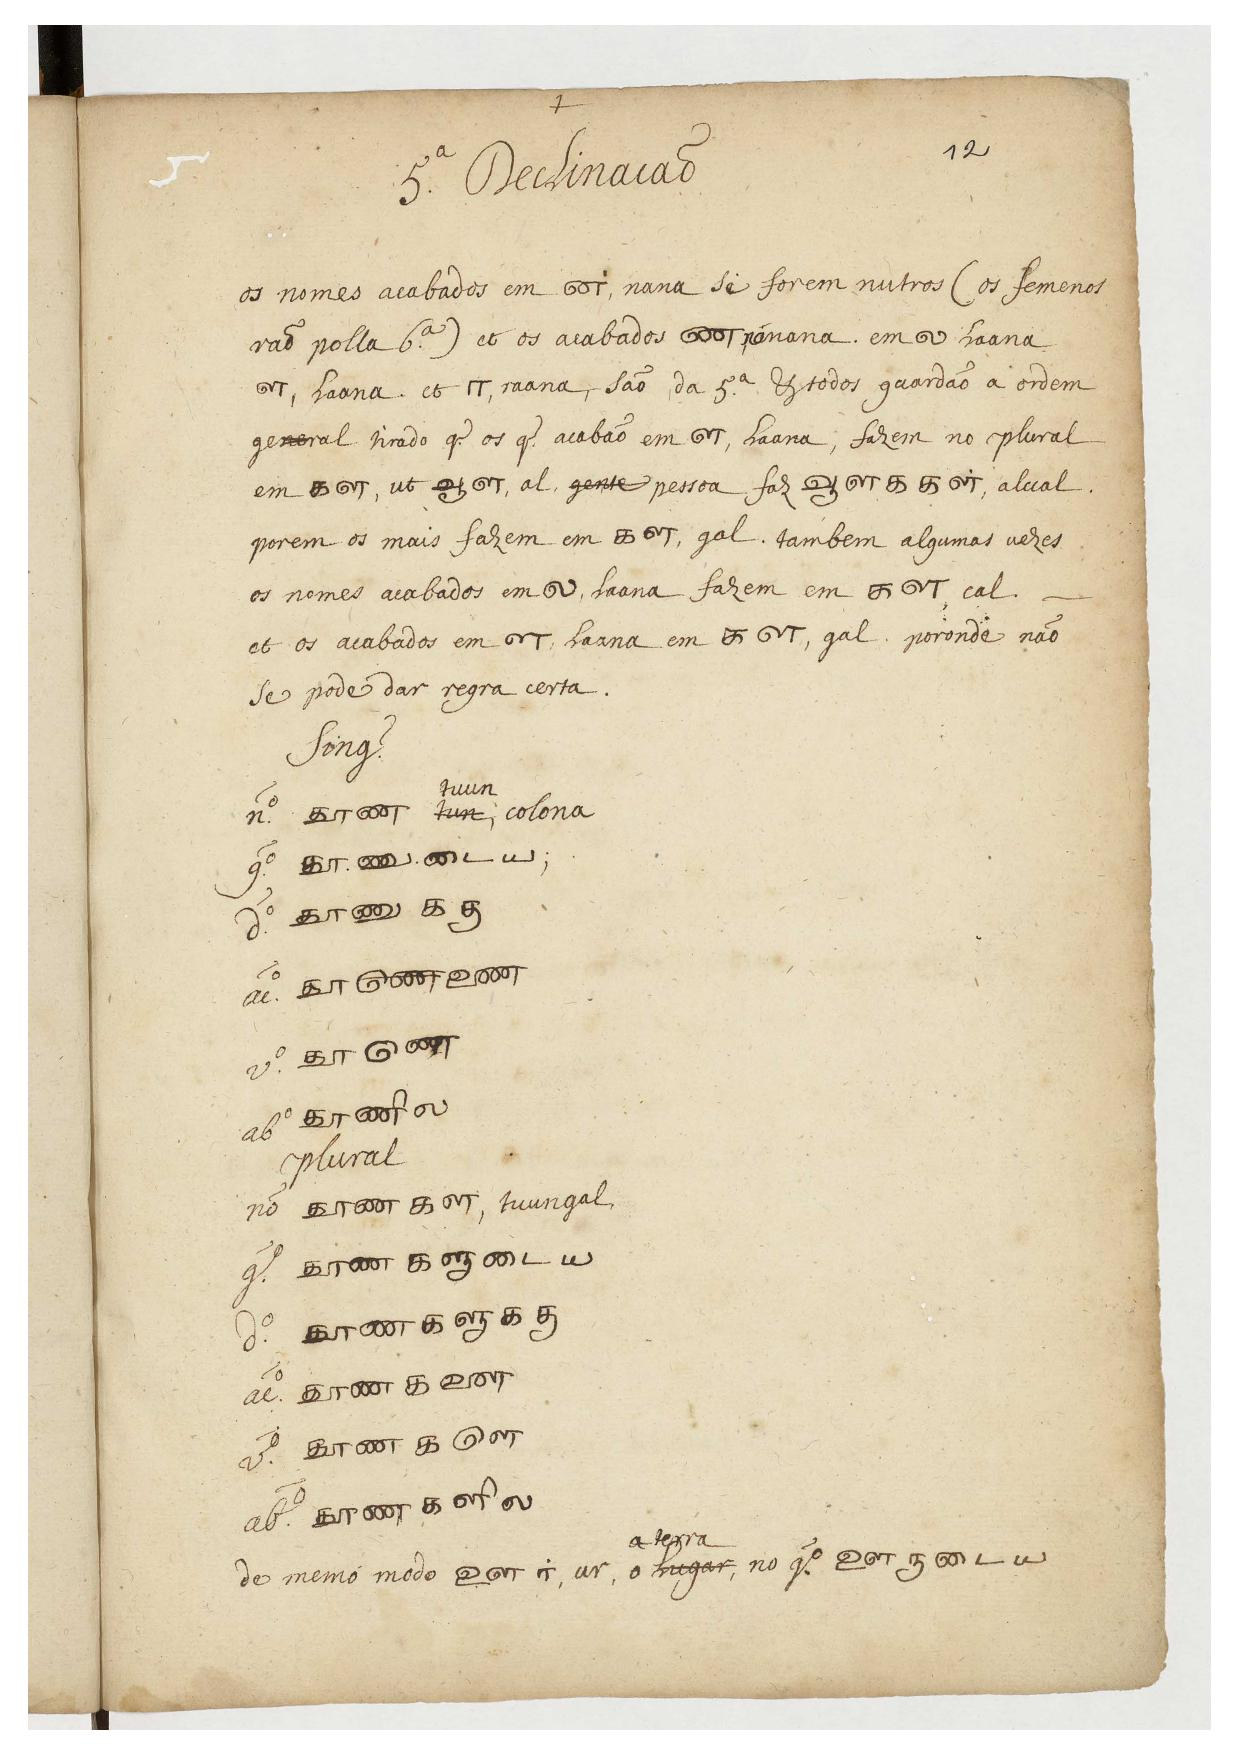
\includegraphics[width=\textwidth]{img-33}}
\newpage
      \chapter*{4ª \sout{\textcolor{gray}{5ª}}Declinacaõ}
    \addcontentsline{toc}{chapter}{4ª \sout{\textcolor{gray}{5ª}}Declinacaõ}
    
      

 Os nome acabados em ம ma, saõ da 4ª declinacaõ
             e no g[enitiv]o do sing[olar]o duas maneiras, ou em உடைய, ou 
	      em தினுடைய, tinudeïa, no plur[al] em கள ut. 
        
      
\begin{tabular}{lllll}
    
        
          Sing. &
          n\textsuperscript{õ} &
          ப.ண.ட.ம &
          pandam &
          fato \\
    
        
    
        
           &
          g\textsuperscript{õ} &
          ப.ண.ட.னு.டை.ய &
          ப.ண.த.தி.னு.டை.ய \\
    
        
    
        
           &
          d\textsuperscript{õ} &
          பணடததுககு \\
    
        
    
        
           &
          ac\textsuperscript{õ} &
          பணடததை \\
    
        
    
        
           &
          v\textsuperscript{õ} &
          பணடத்தெ \\
    
        
    
        
           &
          ab\textsuperscript{õ} &
          பணடததில் \\
    
        
    
        
          plur. &
          n\textsuperscript{õ} &
          பணடஙகள &
          cambugal &
          os paos \\
    
        
    
        
           &
          g\textsuperscript{õ} &
          பணடஙளுடைய &
          cambudeïïa &
          dos paos \\
    
        
    
        
           &
          d\textsuperscript{õ} &
          பணடஙளுககு \\
    
        
    
        
           &
          ac\textsuperscript{õ} &
          பணடஙளை \\
    
        
    
        
           &
          v\textsuperscript{õ} &
          பணடஙளெ \\
    
        
    
        
           &
          ab\textsuperscript{õ} &
          பணடஙளில் \\
    
        
    
      
\end{tabular}
    
      

 De mesmo modo எடம\textbf{edam}, o lugar, பிறகாசம, \textbf{prahatcham},   பிறசாததினுடைய  lume,   செபததினுடைய  oracaõ

      
\newpage
\hypertarget{img-35}{
    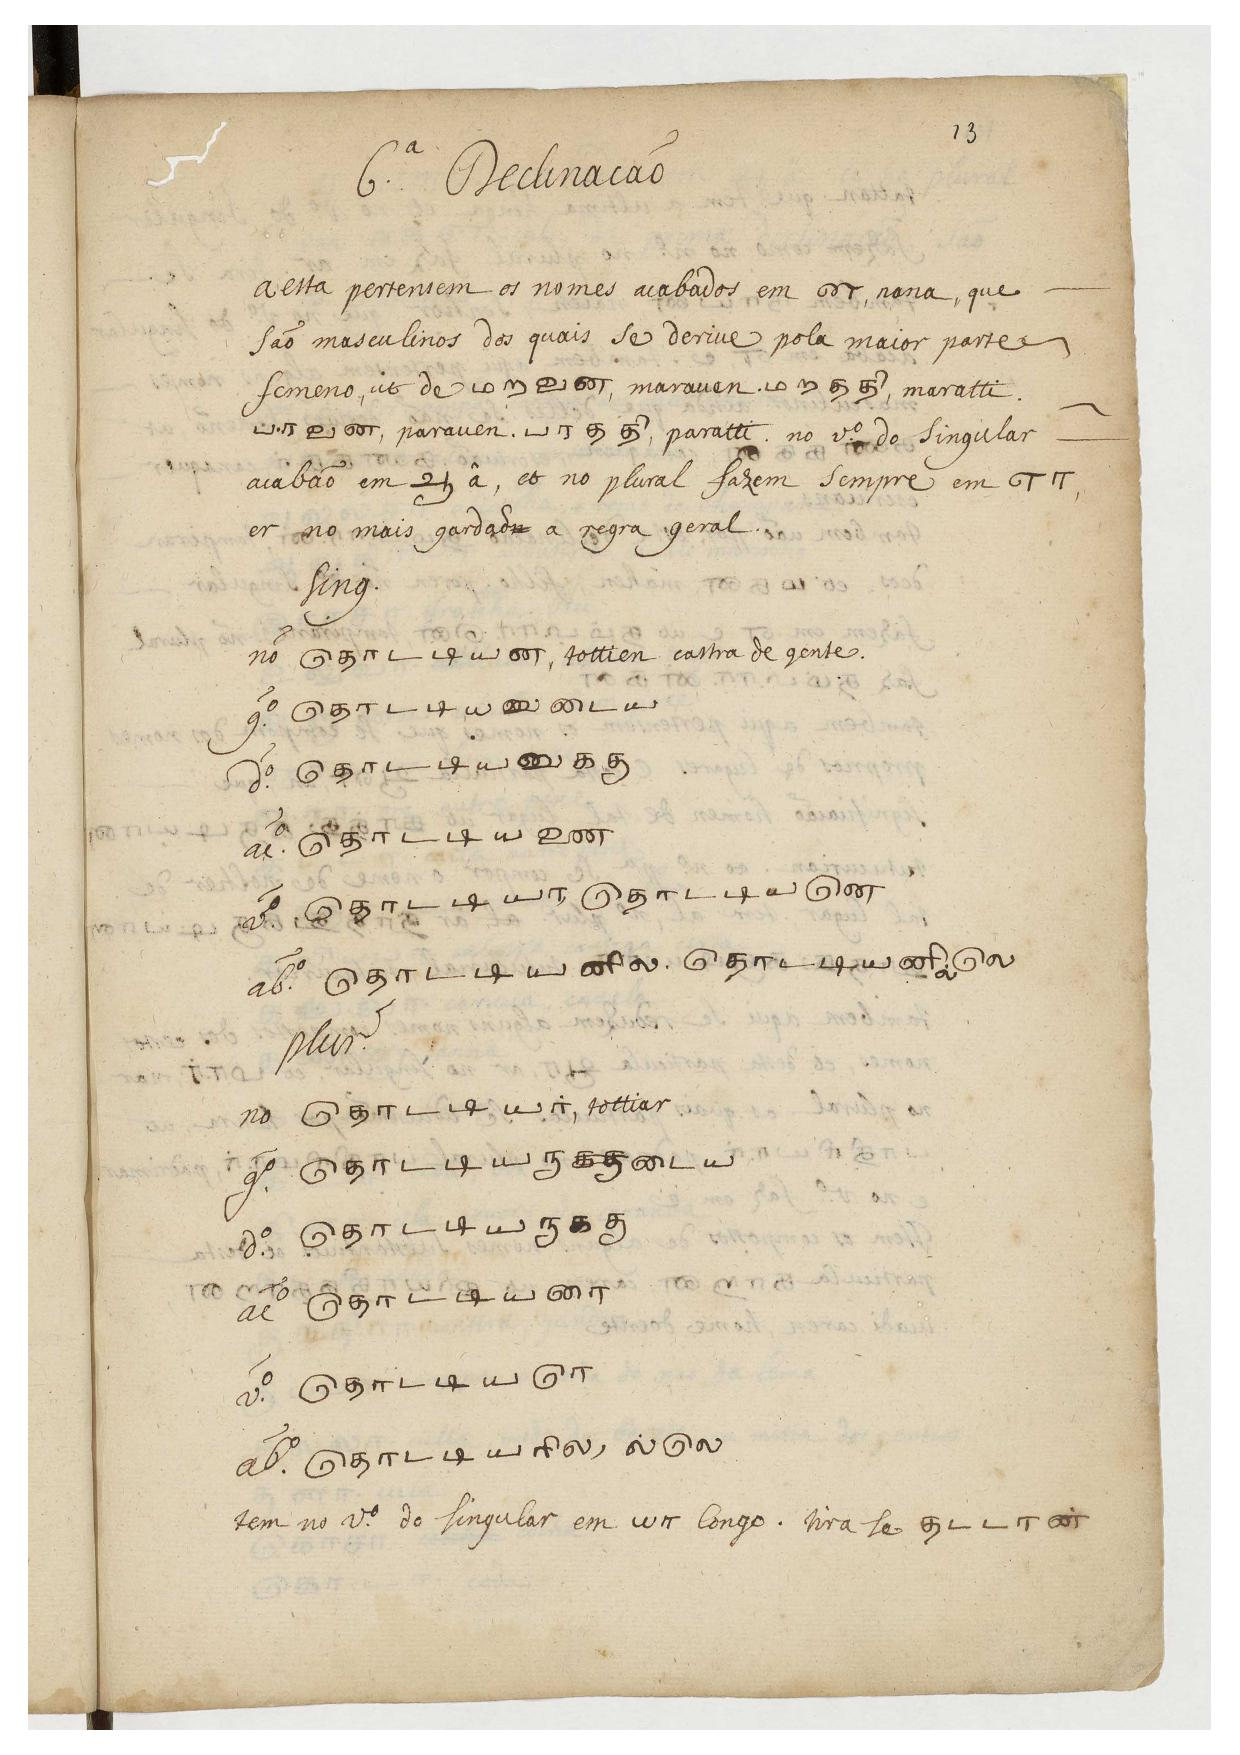
\includegraphics[width=\textwidth]{img-35}}
\newpage
      \chapter*{5ª Declinacaõ}
    \addcontentsline{toc}{chapter}{5ª Declinacaõ}
    
      

 Os nome acabados em ன  nana ser forem neutros (os femenos vaõ polla 6ª) et os acabados ண nánana.  
ஆ â saõ da 1° declinaçaõ no g[enitiv]o do 
            em ல laana, ள laana, et ர raana, saõ da 5ª et todos guardaõ a ordem
            geral tirado q[ue] as q[ue] 
	      acabaõ em ள laana, fazem no plural em கள ut ஆள, al pessoa faz  ஆளககள், alccal porem os mais
            fazem em கள, gal. Tambem algumas vezes os nomes acabados em lb/>em ல laana fazem em fazem em கள, et os 
	     acabados em ள laana em கள, gal poronde naõ
            se pode dar regra certa.
        
      
\begin{tabular}{lllll}
    
        
          Sing. &
          n\textsuperscript{õ} &
          தூண &
          tuun &
          colona \\
    
        
    
        
           &
          g\textsuperscript{õ} &
          தூணுடை.ய \\
    
        
    
        
           &
          d\textsuperscript{õ} &
          தூணுககு \\
    
        
    
        
           &
          ac\textsuperscript{õ} &
          தூணை \\
    
        
    
        
           &
          v\textsuperscript{õ} &
          தூணெ \\
    
        
    
        
           &
          ab\textsuperscript{õ} &
          தூணில \\
    
        
    
        
          plur. &
          n\textsuperscript{õ} &
          தூணகள &
          tungal \\
    
        
    
        
           &
          g\textsuperscript{õ} &
          தூணகளுடை.ய \\
    
        
    
        
           &
          d\textsuperscript{õ} &
          தூணகளுககு \\
    
        
    
        
           &
          ac\textsuperscript{õ} &
          தூணகளை \\
    
        
    
        
           &
          v\textsuperscript{õ} &
          தூணகளெ \\
    
        
    
        
           &
          ab\textsuperscript{õ} &
          தூணகளில \\
    
        
    
      
\end{tabular}
    
      

do mesmo modo ஊர், ur, \sout{\textcolor{gray}{ o  
  lugar}} a terra no g[enitiv]o
	ஊருடைய.
      
\newpage
\hypertarget{img-37}{
    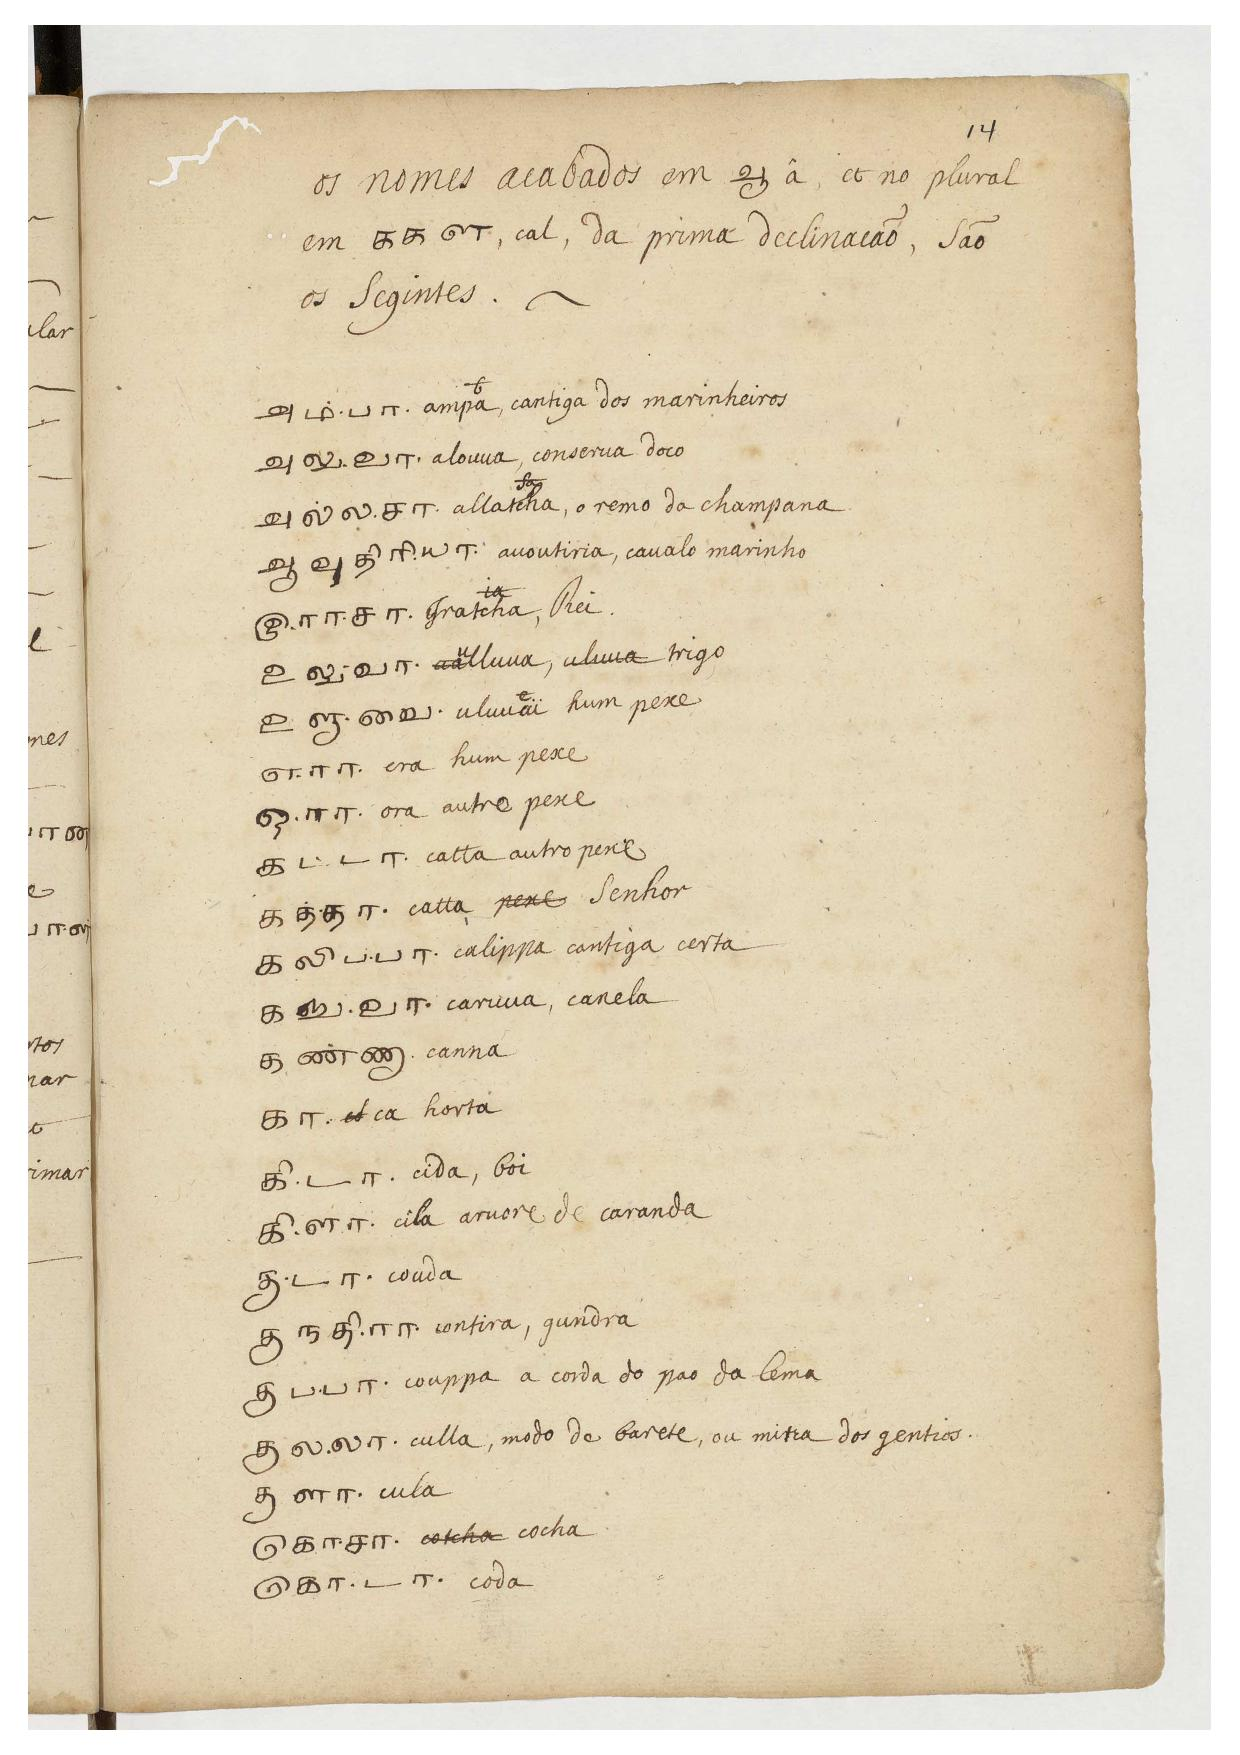
\includegraphics[width=\textwidth]{img-37}}
\newpage
      \chapter*{6ª Declinacaõ}
    \addcontentsline{toc}{chapter}{6ª Declinacaõ}
    
      

 A esta pertenecem os nomes acabados em ன , nana, que saõ masculinos dos quais se
             deriva pola maior parte femeno, ut de மறவன maraven, மறததி maratti acabaõ em ஆ 
            â, et no plural, fazem sempre em எர er no mais gardaõ a regra geral.
        
      
\begin{tabular}{lllll}
    
        
          Sing. &
          n\textsuperscript{õ} &
          தொடடியன &
          totten &
          de gente \\
    
        
    
        
           &
          g\textsuperscript{õ} &
          தொடடியனுடைய \\
    
        
    
        
           &
          d\textsuperscript{õ} &
          தொடடியனுககு \\
    
        
    
        
           &
          ac\textsuperscript{õ} &
          தொடடியனை \\
    
        
    
        
           &
          v\textsuperscript{õ} &
          தொடடியதொடடியனெ \\
    
        
    
        
           &
          ab\textsuperscript{õ} &
          தொடடியனில &
          தொடடியனிலலெ \\
    
        
    
        
          plur. &
          n\textsuperscript{õ} &
          தொடடியர் &
          tottiar \\
    
        
    
        
           &
          g\textsuperscript{õ} &
          தொடடியரு\sout{\textcolor{gray}{ ககுடை.ய}}\textbf{டைய} \\
    
        
    
        
           &
          d\textsuperscript{õ} &
          தொடடியருககு \\
    
        
    
        
           &
          ac\textsuperscript{õ} &
          தொடடியரை \\
    
        
    
        
           &
          vo\textsuperscript{õ} &
          தொடடியரெ. \\
    
        
    
        
           &
          ab\textsuperscript{õ} &
          தொடடியரில, ல்லெ \\
    
        
    
      
\end{tabular}
    
      

 tem no v[ocativ]o do singular em யா longo. Tira le தடடான்.
      
\newpage
\hypertarget{img-39}{
    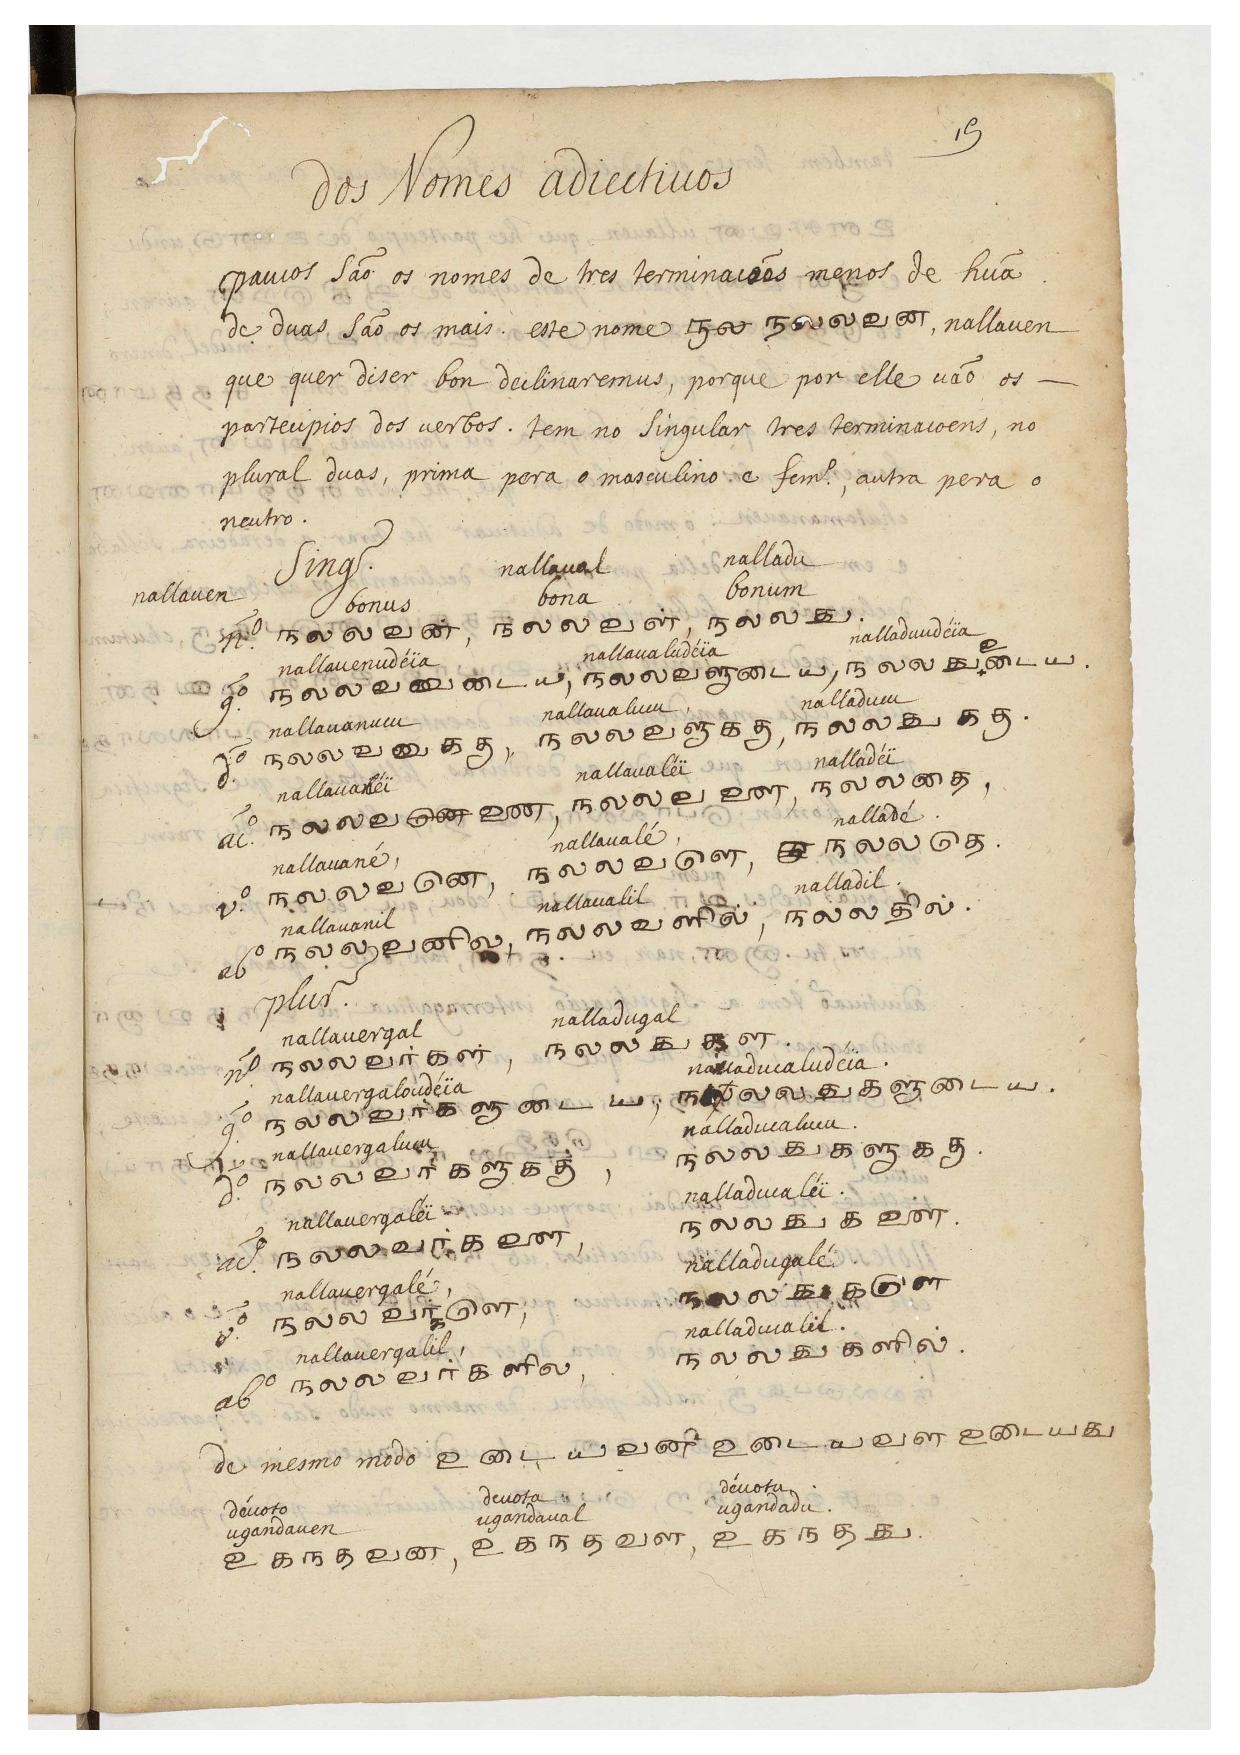
\includegraphics[width=\textwidth]{img-39}}
\newpage
      

 tattan que tem a ultima lunga et no v[ocativ]o do singular fazem como no
         n[ominativ]o no plural faz em ar. Tira se tàmbem நாய்ன, naïen, senhor que no 
        v[ocativ]o do singular acaba em எ tambem aqui pertensem alguns nomes 
         masculinos ainda que delles se naõ derive femenõ ut கணககன canaquen escrivaõ
        	    கனககர், canaquer, escrivans.
        	     Tambem naõ por esta declinacaõ தம்பிரான், tampiran deos et மகன, mahen, filho.
                Poren nõ v[ocativ]o singular fazem em எ e ut தம்பிரானெ, tampirane, nõ plural faz 
        	   தம்பிரான்கள். 
        	    Tambem aqui pertensem os nomes que se compom dos nomes proprios de lugares e
         desta particula ஆன, an que significaõ homen de tal lugar ut தூத்துக்குடியாள, 
    தூத்துக்குடியார. tuttucurial, tuttucuriar.
Tambem aqui se reduzem alguns nomes compostos dos certos nomes et desta  particula ஆர, ar no singular et மார no plural as quais pariculas se diuntaõ por 
honra, no பாதிரியார் padriar no plural பாதிரிமார் padrimar e no v[ocativ]o faz em e.
Item os compostos de alguns nomes substantivos et desta particula காறன, caren, 
ut வியாதிக்காறன, viadi caren, home doente. 
	
      
\newpage
\hypertarget{img-41}{
    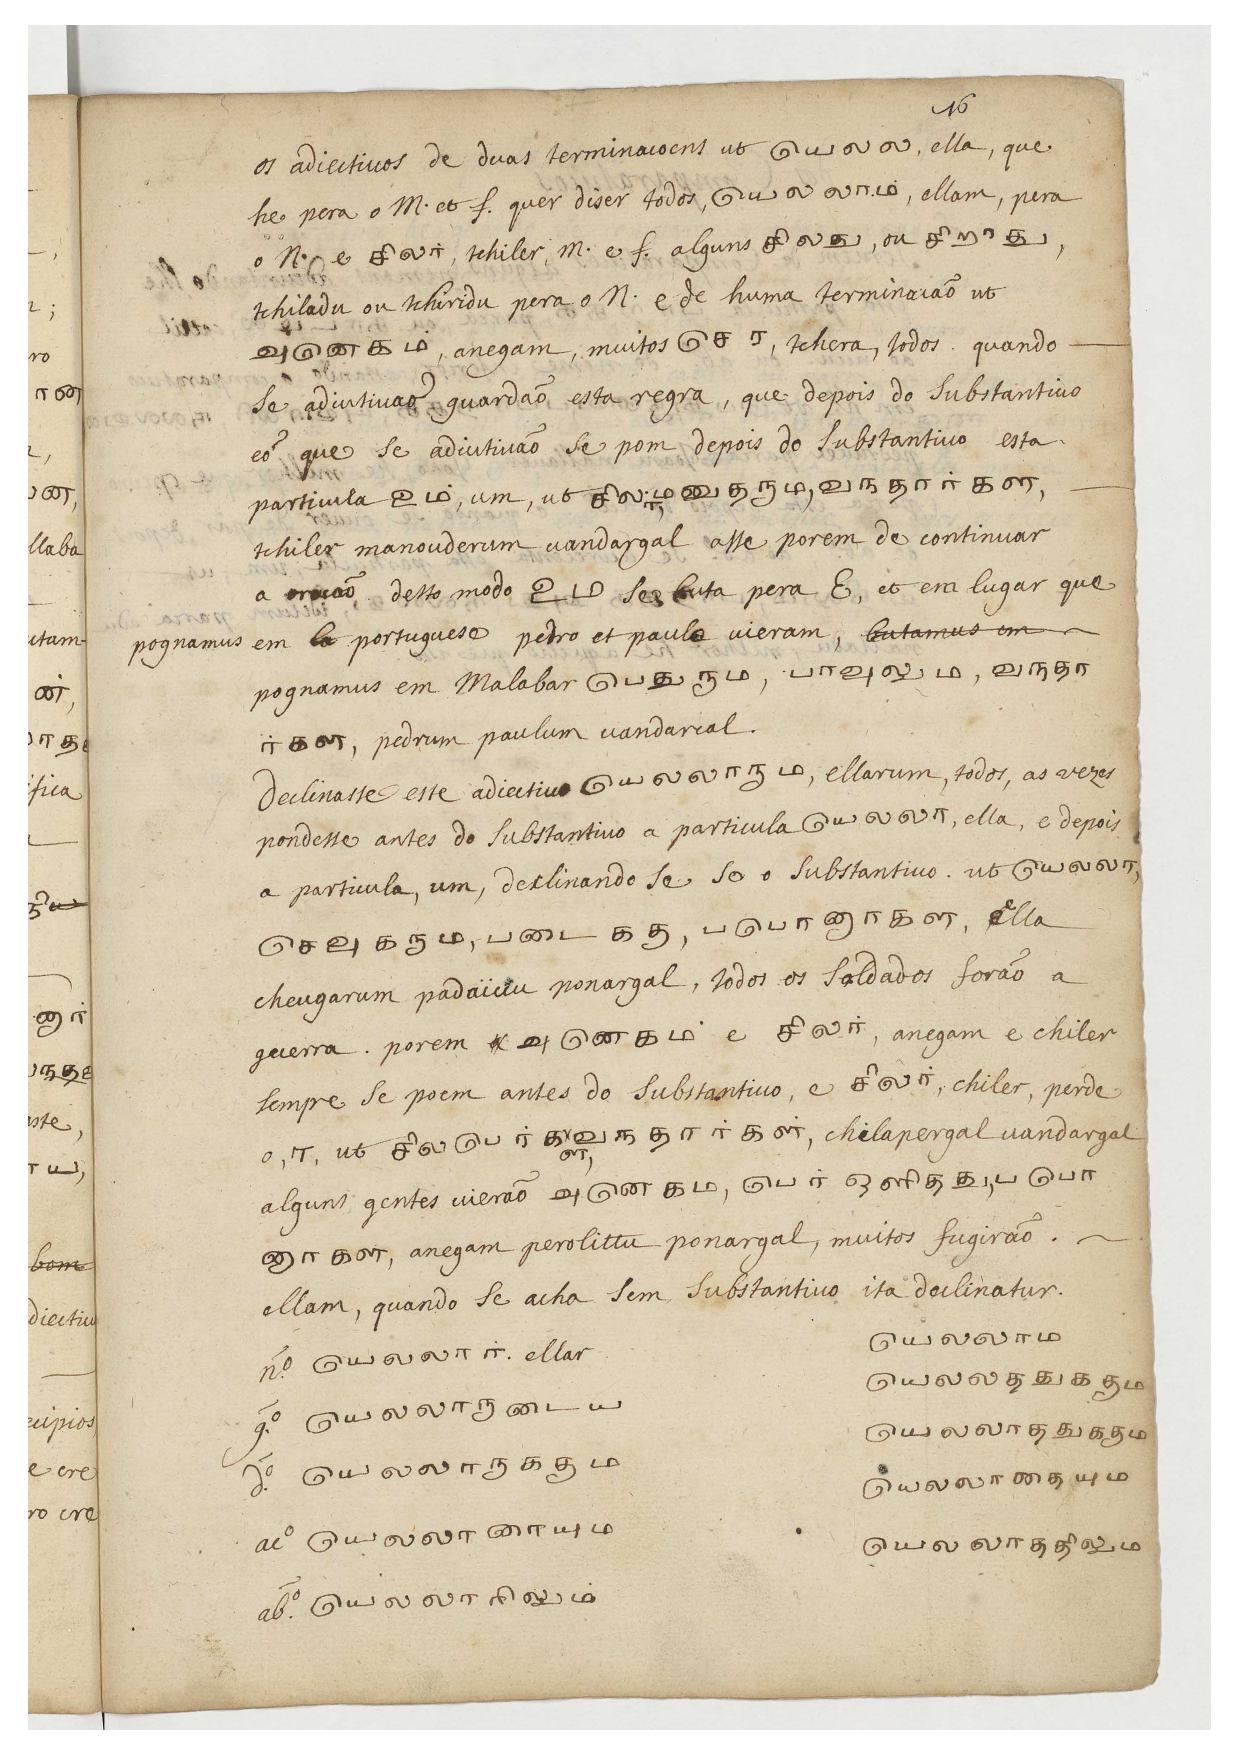
\includegraphics[width=\textwidth]{img-41}}
\newpage
      

os nomes acabados em ஆ â et no plural em ககள, cal, da prima declinacaõ, saõ os 
             segintes.
        
      
\begin{tabular}{lll}
    
        
           &
          அம்.பா &
          am\sout{\textcolor{gray}{b}}\textbf{p}pa, cantiga dos 
		marinheiros \\
    
        
    
        
           &
          அலுவா &
          aluova, conserva doco \\
    
        
    
        
           &
          அல்லசா &
          allatcha, o remo da champana \\
    
        
    
        
           &
          ஆவுதிரியா &
          avoutiria, canale marinho \\
    
        
    
        
           &
          இரசா &
          jratcha, Rei \\
    
        
    
        
           &
          உலுவ &
          ulluva,\sout{\textcolor{gray}{uluva}}, trigo \\
    
        
    
        
           &
          உளுவை &
          uluvai, hum peixe \\
    
        
    
        
           &
          எரா &
          era, hum peixe \\
    
        
    
        
           &
          ஒரா &
          ora, outro peixe \\
    
        
    
        
           &
          கடடா &
          catta, outro peixe \\
    
        
    
        
           &
          கததா &
          catta \sout{\textcolor{gray}{peixe}}, Senhor \\
    
        
    
        
           &
          கலிபபா &
          calippa, cantiga certa \\
    
        
    
        
           &
          கறுவா &
          caruca, canela \\
    
        
    
        
           &
          கணணா &
          canna \\
    
        
    
        
           &
          கா &
          ca, horta \\
    
        
    
        
           &
          ஆவுதிரியா &
          avoutiria	canale marinho \\
    
        
    
        
           &
          கிடா &
          cida, boi \\
    
        
    
        
           &
          சிளா &
          cila, arvore de caranda \\
    
        
    
        
           &
          குடா &
          couda \\
    
        
    
        
           &
          குநதிரா &
          contira, gundra \\
    
        
    
        
           &
          குபபா &
          couppa, a corda do pao da lema \\
    
        
    
        
           &
          குலலா &
          culla, 	modo de barete, ou mitra dos gentios \\
    
        
    
        
           &
          குளா &
          cula \\
    
        
    
        
           &
          கொசா &
          
            \sout{\textcolor{gray}{cotcha}}
            \textbf{cocha}
           \\
    
        
    
        
           &
          கொடா &
          coda \\
    
        
    
      
\end{tabular}
    
      
\newpage
\hypertarget{img-43}{
    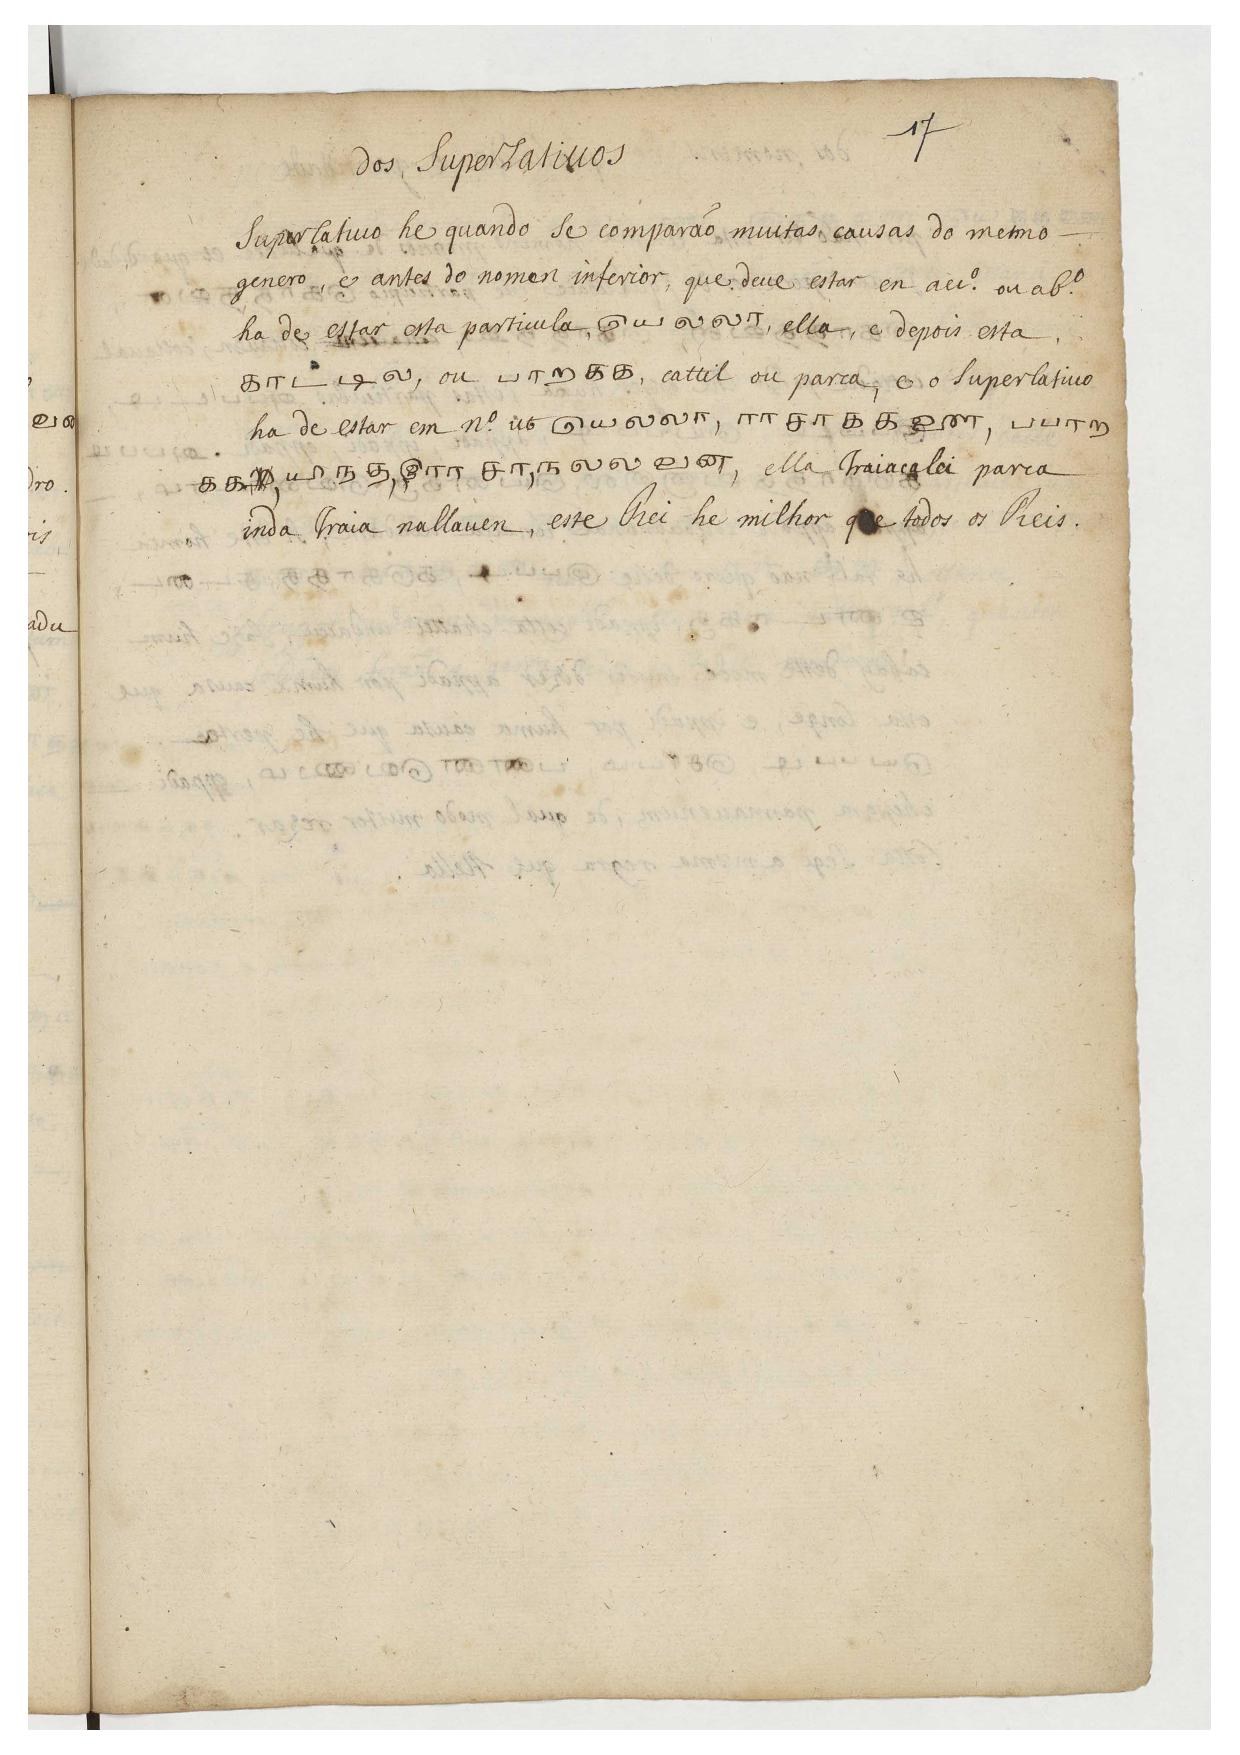
\includegraphics[width=\textwidth]{img-43}}
\newpage
      \chapter*{dos Nomes adiectivos}
    \addcontentsline{toc}{chapter}{dos Nomes adiectivos}
    
      

 pouco saõ os nomes de tres terminacaõs menos de huã de duas saõ os 
mais. Este 
 nome \sout{\textcolor{gray}{நல}} ஆ நலலவன nallaven, que quer diser bon declinaremus, porque por elle vaõ os 
partecipios dos verbos. Tem no singular tres terminacoens, no plural duas, prima 
pero o masculino e fem(inin)o, outra pera o neutro.
        
      
\begin{tabular}{lllll}
    
          
            Sing. &
            n\textsuperscript{õ} &
            bonus &
            bona &
            bonum \\
    
          
    
          
            நலலவன் &
             நலலவள் &
             நலலது \\
    
          
    
          
            nallavenudeïa &
            nallaveludeïa &
            nalladuudeïa \\
    
          
    
          
            Sing. &
            g\textsuperscript{õ} &
            நலலவனுடைய &
            நலலவளுடைய &
            நலலது உடைய \\
    
          
    
          
            nallavanucu &
            nallavalucu &
            nalladucu \\
    
          
    
          
            d\textsuperscript{õ} &
            நலலவனுககு &
            நலலவளுககு &
            நலலதுககு \\
    
          
    
          
            nallavaneï &
            nallavaleï &
            nalladai \\
    
          
    
          
            ac\textsuperscript{õ} &
            நலலவனை &
            நலலவளை &
            நலலதை \\
    
          
    
          
            nallavané &
            nallavalé &
            nalladé \\
    
          
    
          
            v\textsuperscript{õ} &
            நலலவனெ &
            நலலவளெ &
            நலலதெ \\
    
          
    
          
            nallavanil &
            nallavalil &
            nalladil \\
    
          
    
          
            ab\textsuperscript{õ} &
            நலலவனில் &
            நலலவளில் &
            நலலதில் \\
    
          
    
          
            plur &
            nallavergal &
            nalladugal \\
    
          
    
          
            n\textsuperscript{õ} &
            நலலவவர்கள் &
            நலலதுகள் \\
    
          
    
          
            plur &
            nallavergaloudeïa &
            nallavaducaludeïa \\
    
          
    
          
            g\textsuperscript{õ} &
            நலலவவர்களுடைய &
            நலலவதுகளுடைய \\
    
          
    
          
            nallavergalucu &
            nallavaducalucu \\
    
          
    
          
            d\textsuperscript{õ} &
            நலலவர்களுககு &
            நலலவதுகளுககு \\
    
          
    
          
            nallavergaleï &
            nallavadugaleï \\
    
          
    
          
            ac\textsuperscript{õ} &
            நலலவவர்களை &
            நலலவதுகளை \\
    
          
    
          
            nallavergal[ &
            nallavadugalé \\
    
          
    
          
            v\textsuperscript{õ} &
            நலலவவர்களெ &
            நலலவதுகளெ \\
    
          
    
          
            nallavergalil &
            nallavaducalil \\
    
          
    
          
            ab\textsuperscript{õ} &
            நலலவவர்களில &
            நலலவதுகளில் \\
    
          
    
      
\end{tabular}
    
      

de mesmo modo உடையவனஉடையவளஉடையது
      
\newpage
\hypertarget{img-45}{
    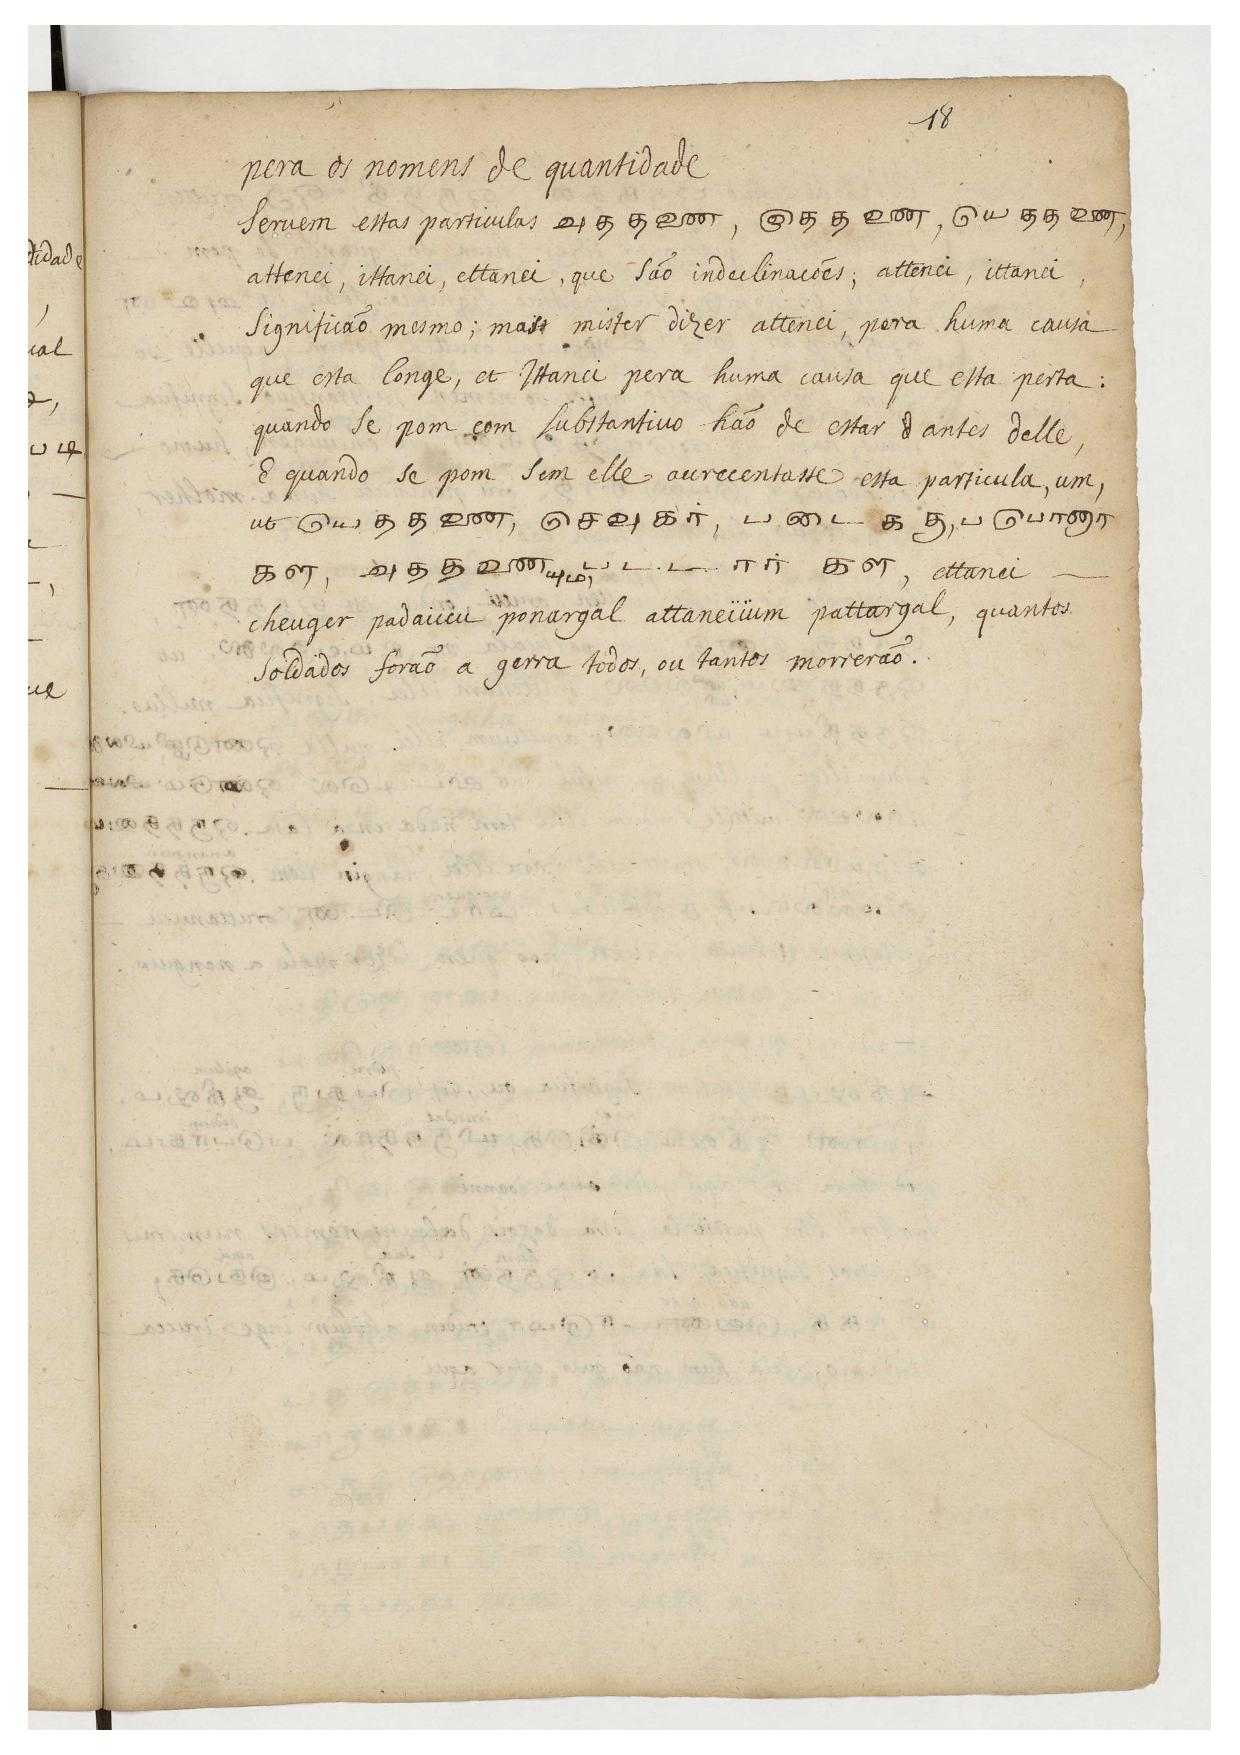
\includegraphics[width=\textwidth]{img-45}}
\newpage
      

tambem serve de adiectivos os substantivos essa particula உளளவன, ullaven, que 
he participio de உணடு undu et ஆனவன, anaven, participio de ஆகிறென், acren; ut 
மிதிலுளளவன, முதல் உளளவன mudel, dinero, ullaven, homẽ que tem. Homẽ que tem dinero. 
சுததமான chutamana quer dizer limpeza ou sanctidade, அவன, aven, homen, ambos iuntos, homen que he iusto சுததமானவன, chutamanaven. O modo de adïïtivar he tirar 
a dearadeira sillaba e em lugar della por o pronome declinado os ambos, polla declinaçaõ do substantivo ut சுததமான,பெதுரு chutamana pedru, sanctu pedru, வியாதி, 
உளள, மனதன், viadi ulla manuden, homen doente. Tirase பொலலாத[வன] pollādaven, 
que perde as derdeiras sillabas, e que significa mao homen; பொலலா,மனுதி polla 
manudi, roim molhêr.
Algũas vezes ஆர் (quem) ar, யெது, edou, qui et os pronomes நி, ni, vos, tu, னான, 
nan, eu, தான, tan, elle quando see adiuticaõ tem a significaõ interrogativa, ut 
வனதவனார் vandavanar, quem he que ia vi, ou quem he o que veïo வநத[-]நியென,வனதாய, 
vandava nien vandaï, tu que vieste, pera que vieste? விட\sout{\textcolor{gray}{டிலெ}}டுககு நி, யென, வந்தாய, 
\sout{\textcolor{gray}{vittile}} vittucu ni en vandaï, porque viestes [ora a casa]? 
Notesse que nestes adiectivos, ut, நலலவன, nallaven, bom, esta inserrado o substantivo que he அவன, aven, e o adiectivo que he nalla, unde pera dizer pedro 
bom, dize\sout{\textcolor{gray}{ra}}mos, நலல,பெதுரு, nalla pedru, do mesmo modo saõ os partecipios ut 
விசுவதிககிறவன, vichuvadiccraven, pessoa que cre e விசுவதிககிற,பெதுரு, vichuvadiccra 
pedru, pedro cre.

      
\newpage
\hypertarget{img-47}{
    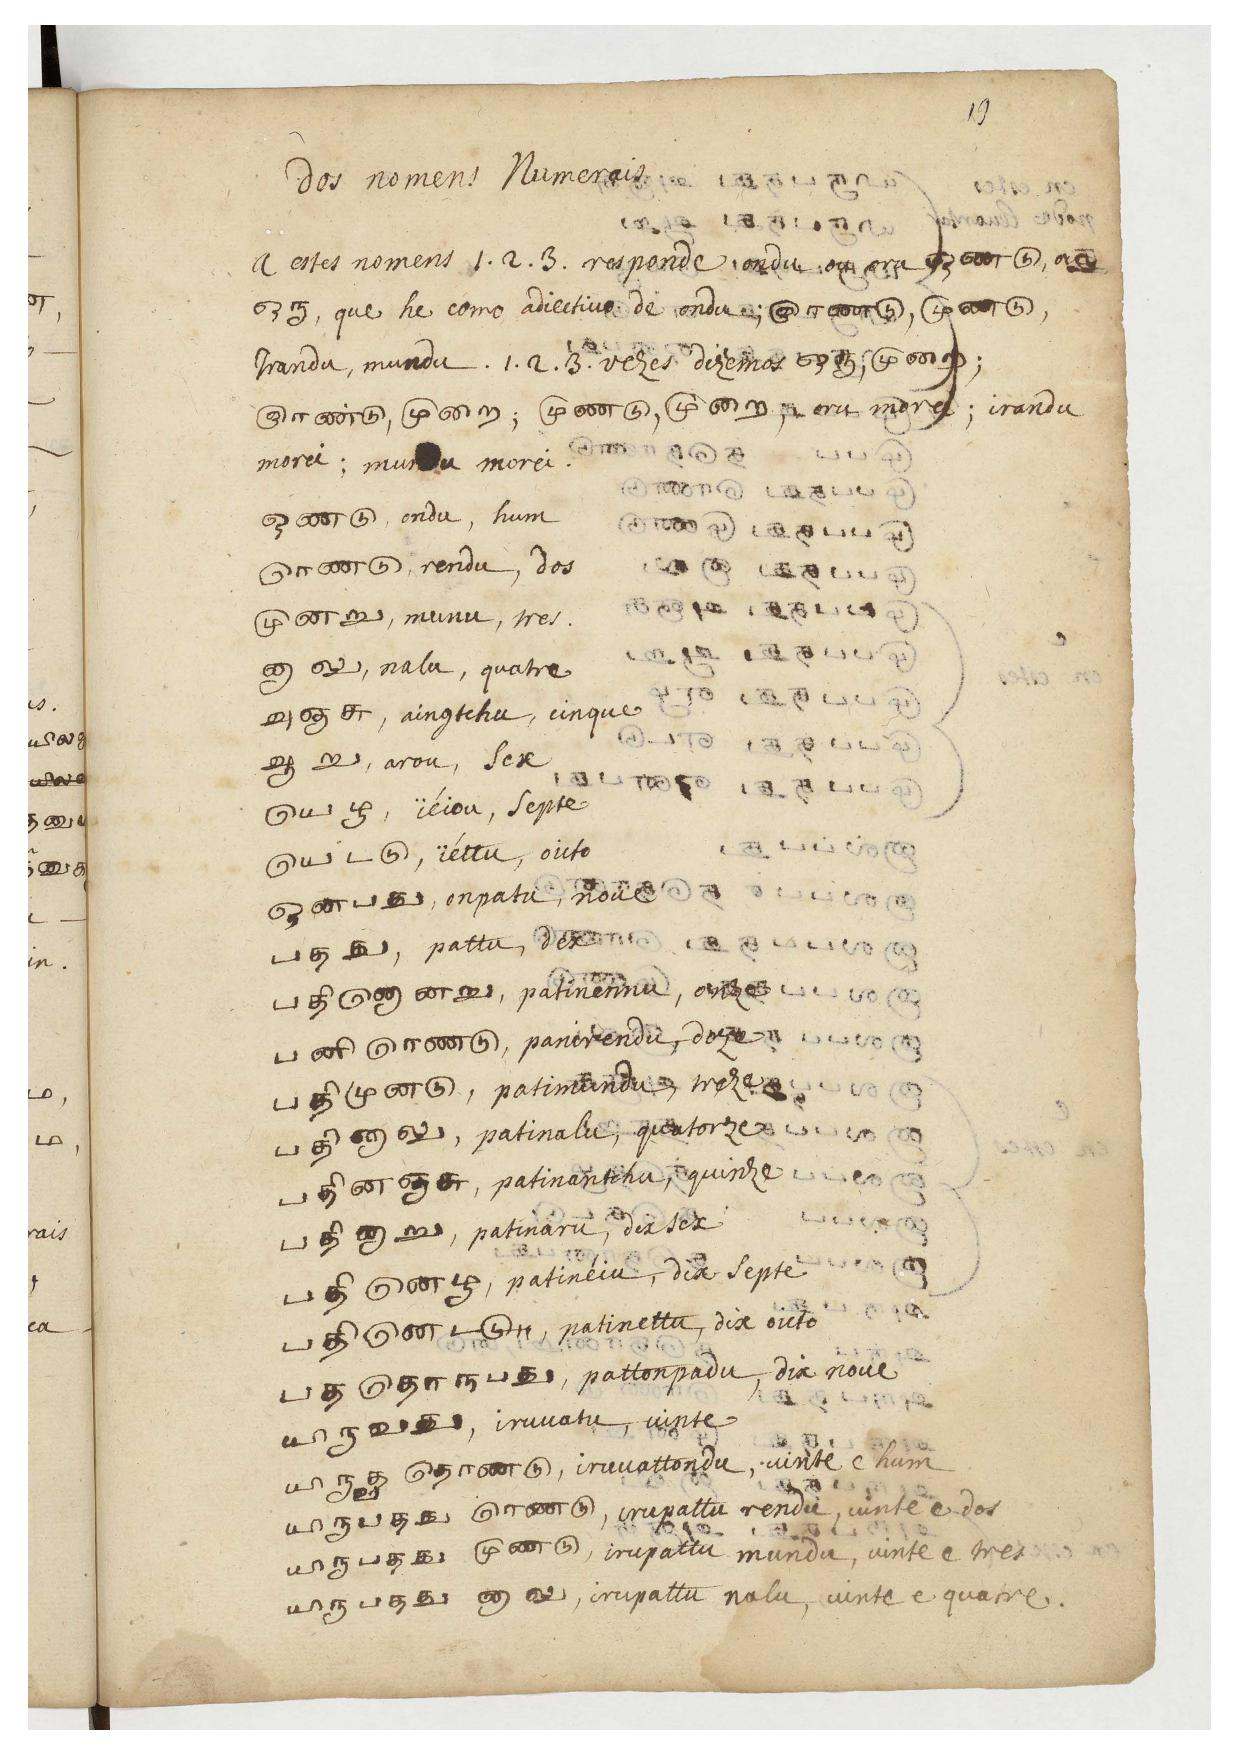
\includegraphics[width=\textwidth]{img-47}}
\newpage
      

os adiectivos de duas terminacoens ut யெலல, ella, que he pera o m. et f. quer 
diser todos, யெலலாம, ellam, per o n. e சிலர், tchiler, m. e f. alguns சிலது, ou 
சிறாது, tchiladu ou tchiridu per o n. e de huma terminacaõ ut அனெகம, anegam, 
muitos, செர, tchera, todos. Quando se adiutivaõ guardaõ esta regra, que depois do 
substantivo cõ que se adiutivaõ se pom depois do substantivo esta particula உம், 
um, ut சிலாமனுதரும, உநதார்கள, tchiler manouderum vandurgal, [asse] porem de continuar 
a oracaõ, desso modo உம se [luta] per E, et em lugar que pongamos em la portuguesa 
pedro et paulo vieram, \sout{\textcolor{gray}{lutamus em}}
pognamus em Malabar பெதுரும, பாவுலும, வநதார்கள, pedrum pavulum vandarcal. 
Declinasse esse adiectivo யெலலாரும, ellarum, todos, as vezes pondesse antes do 
substantivo a particula யெலலா, ella, e depois a particula, um, declinando se so 
o substantivo ut யெலலா, செவுகரும, படைககு, பபொனாரகள, ella chevugarum padaïdu 
ponargal. Todos os sabados forão a guerra. Porem அனெகம் e சிலர், anegam e chiler 
sempre se poem antes do substantivo, e சிலர், chiler, perde o, ர, ut, சிலபெர்கள, வந்தர்கள், chilapergal vandargal, alguns gentes vieraõ அனெகம, பெர், ஒளிதது,பபொனாகள, 
anegam perolittu ponargal, muitos fugiraõ.
Ellam, quando se acha sem substantivo ita declinatur
	
      
\begin{tabular}{llll}
    
        
          n\textsuperscript{õ} &
          எலலார் &
          ellar &
          யெலலாம \\
    
        
    
        
          g\textsuperscript{õ} &
          எலலாருடைய &
          
            \textcolor{purple}{¿}யெலலாததுககும\textcolor{purple}{?}
           \\
    
        
    
        
          d\textsuperscript{õ} &
          எலலாருககும &
          யெலலாததுககும \\
    
        
    
        
          ac\textsuperscript{õ} &
          எலலாரையும &
          ellar &
          யெலலாதையும \\
    
        
    
        
          ab\textsuperscript{õ} &
          எலலாரிலும் &
          ellar &
          யெலலாததிலும \\
    
        
    
      
\end{tabular}
    
      
\newpage
\hypertarget{img-49}{
    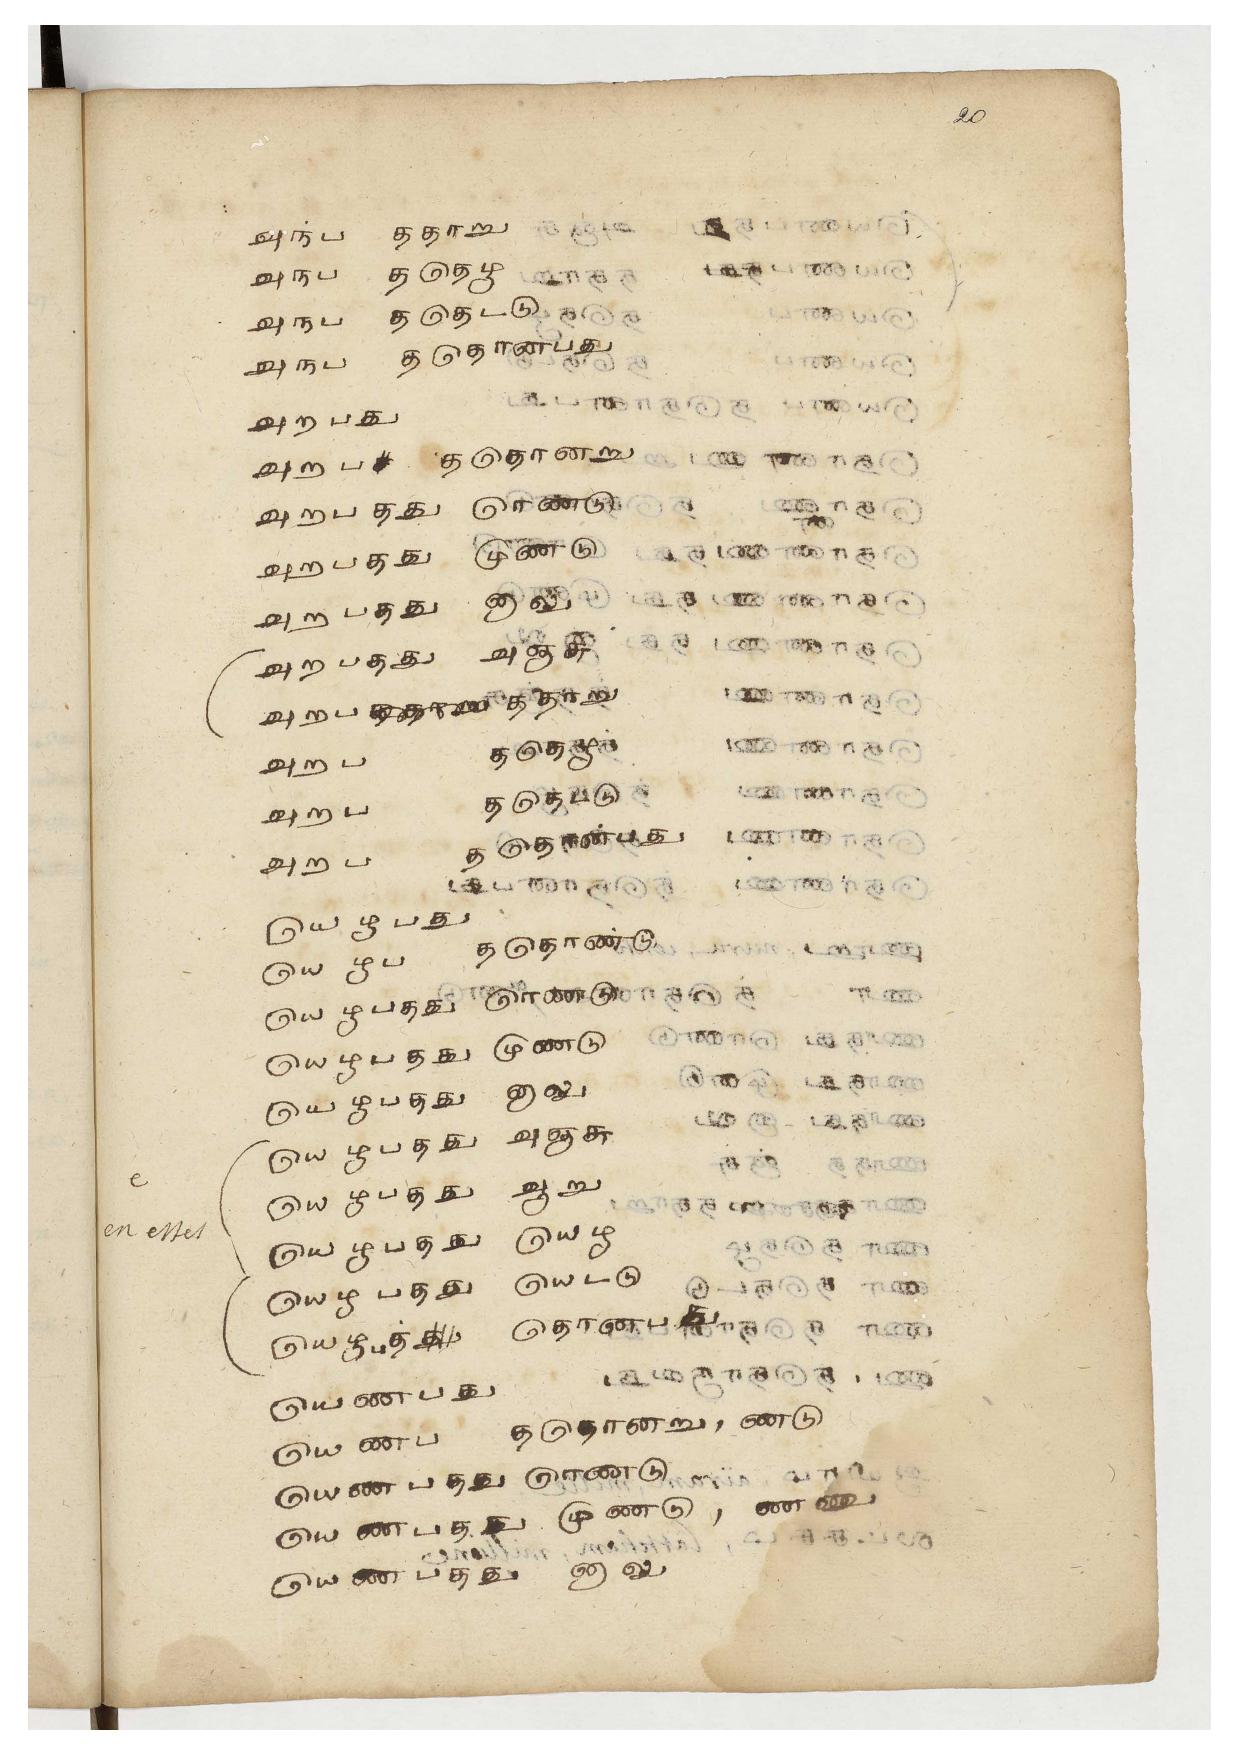
\includegraphics[width=\textwidth]{img-49}}
\newpage
      \chapter*{dos Comparativos}
    \addcontentsline{toc}{chapter}{dos Comparativos}
    
      

Servem dos comparativos alguns nomens adiuntando lhe essa particula பாறகக, parca, 
ou காடடில, cattil ao acc(usativ)o ou ab(lativ)o do nome inferior, estando o 
comparativo em n(ominativ)o ut பெதுருவை,பபாறகக, யுவானி, நலலவன pedruvei parca Joani 
nallaven, Joao he melhor que pedro, parca esta depois de acc(usativ)o e quando se 
ouver de pâr depois do ab(lativ)o se accrecenta esta particula, um ut யிதிலும், 
பாறகக, அது, நலலது, idilum parca adu nalladu, melhor he aquello que isto. 
	
      
\newpage
\hypertarget{img-51}{
    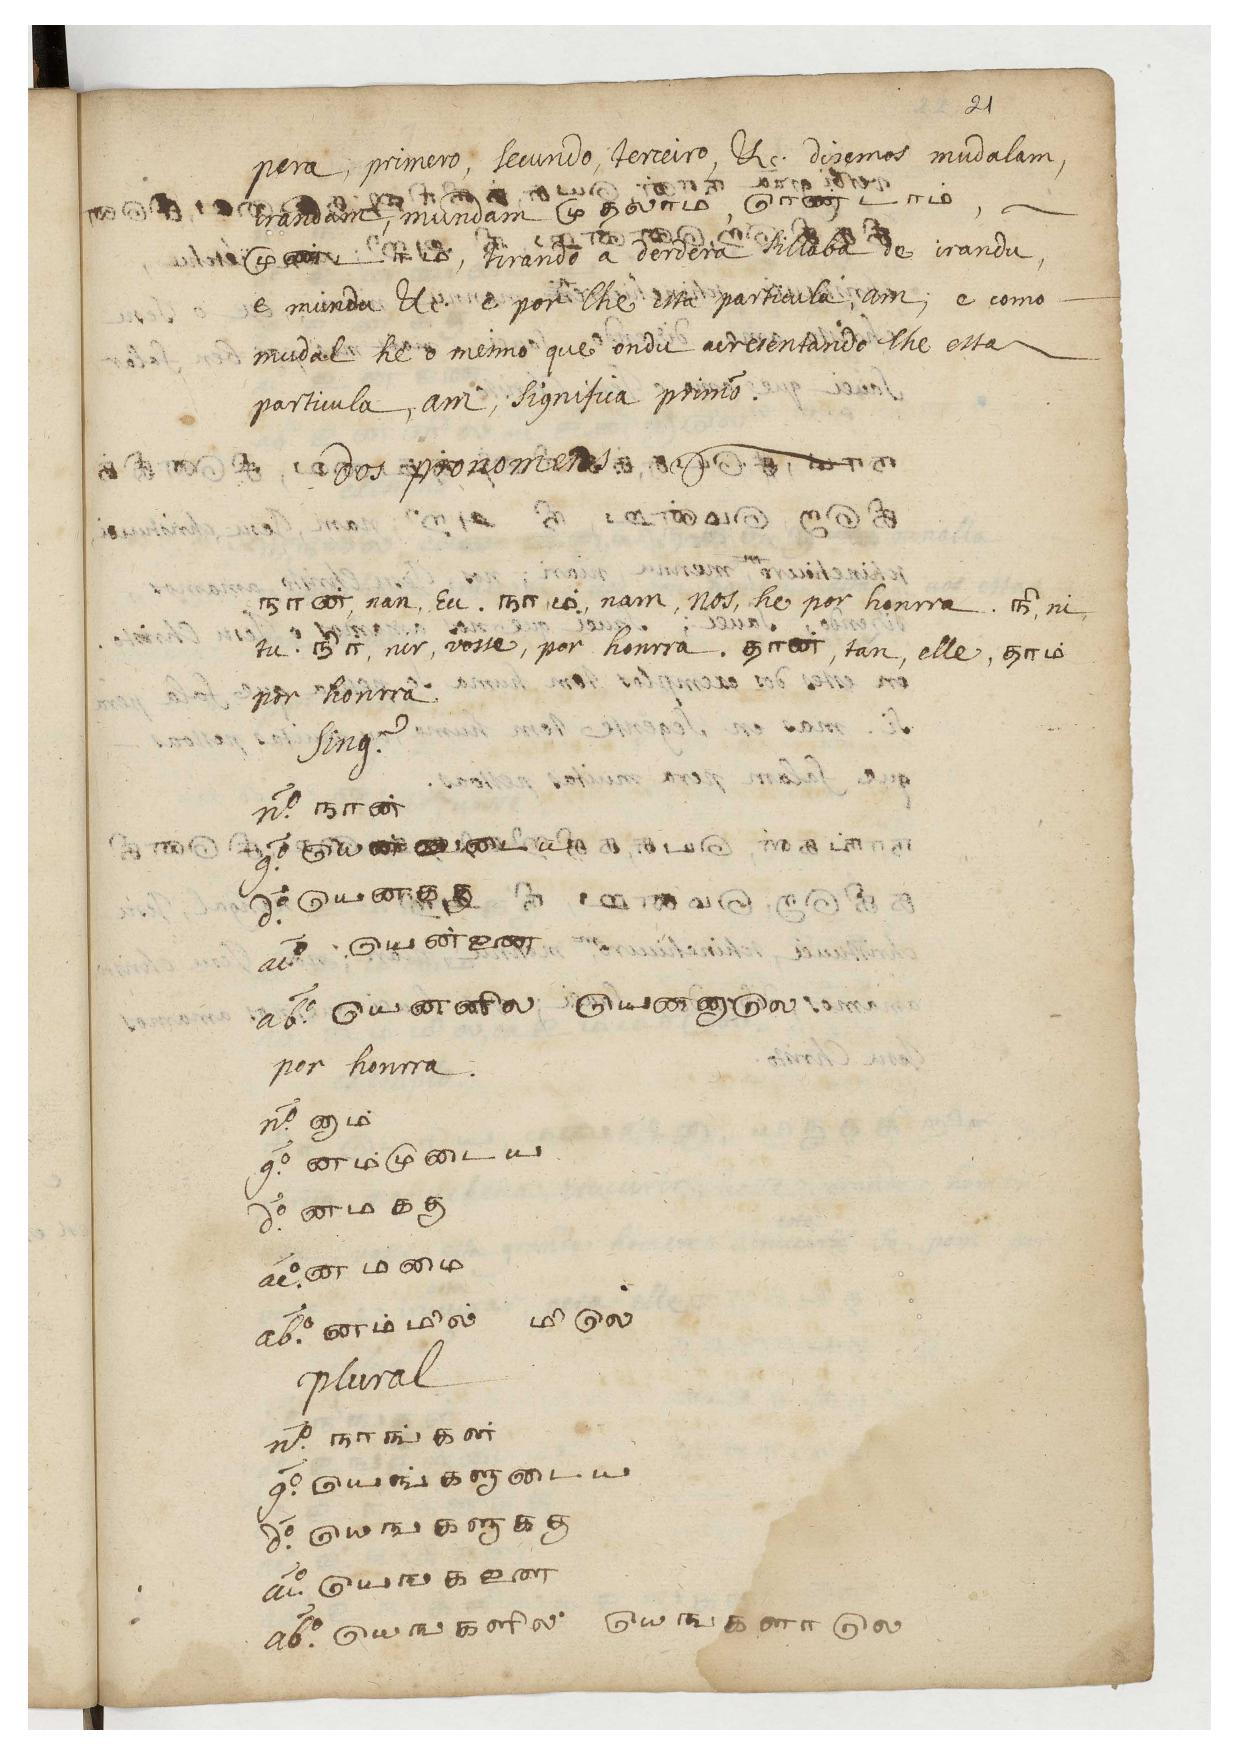
\includegraphics[width=\textwidth]{img-51}}
\newpage
      \chapter*{dos Superaltivos}
    \addcontentsline{toc}{chapter}{dos Superaltivos}
    
      

Superlativo he quando se comparaõ muitas causas do mesmo genero e antes do nomes 	
inferor, que deve estar en acc(usatv)o ou ab(lativ)o ha de ester esta particula 	
யெலலா	ella e depois esta காடடில, ou பாறகக cattil ou parca, e o superlativo ha de 
estar em n(ominativ)o ut யெலலா, ராசாககளை, பபாறகக, யிநத, இராசா, நலலவன, ella 	
Jraicalai parca inda Jraia nallaven, esse Rei he milhor que todos os Reis.
		
      
\newpage
\hypertarget{img-53}{
    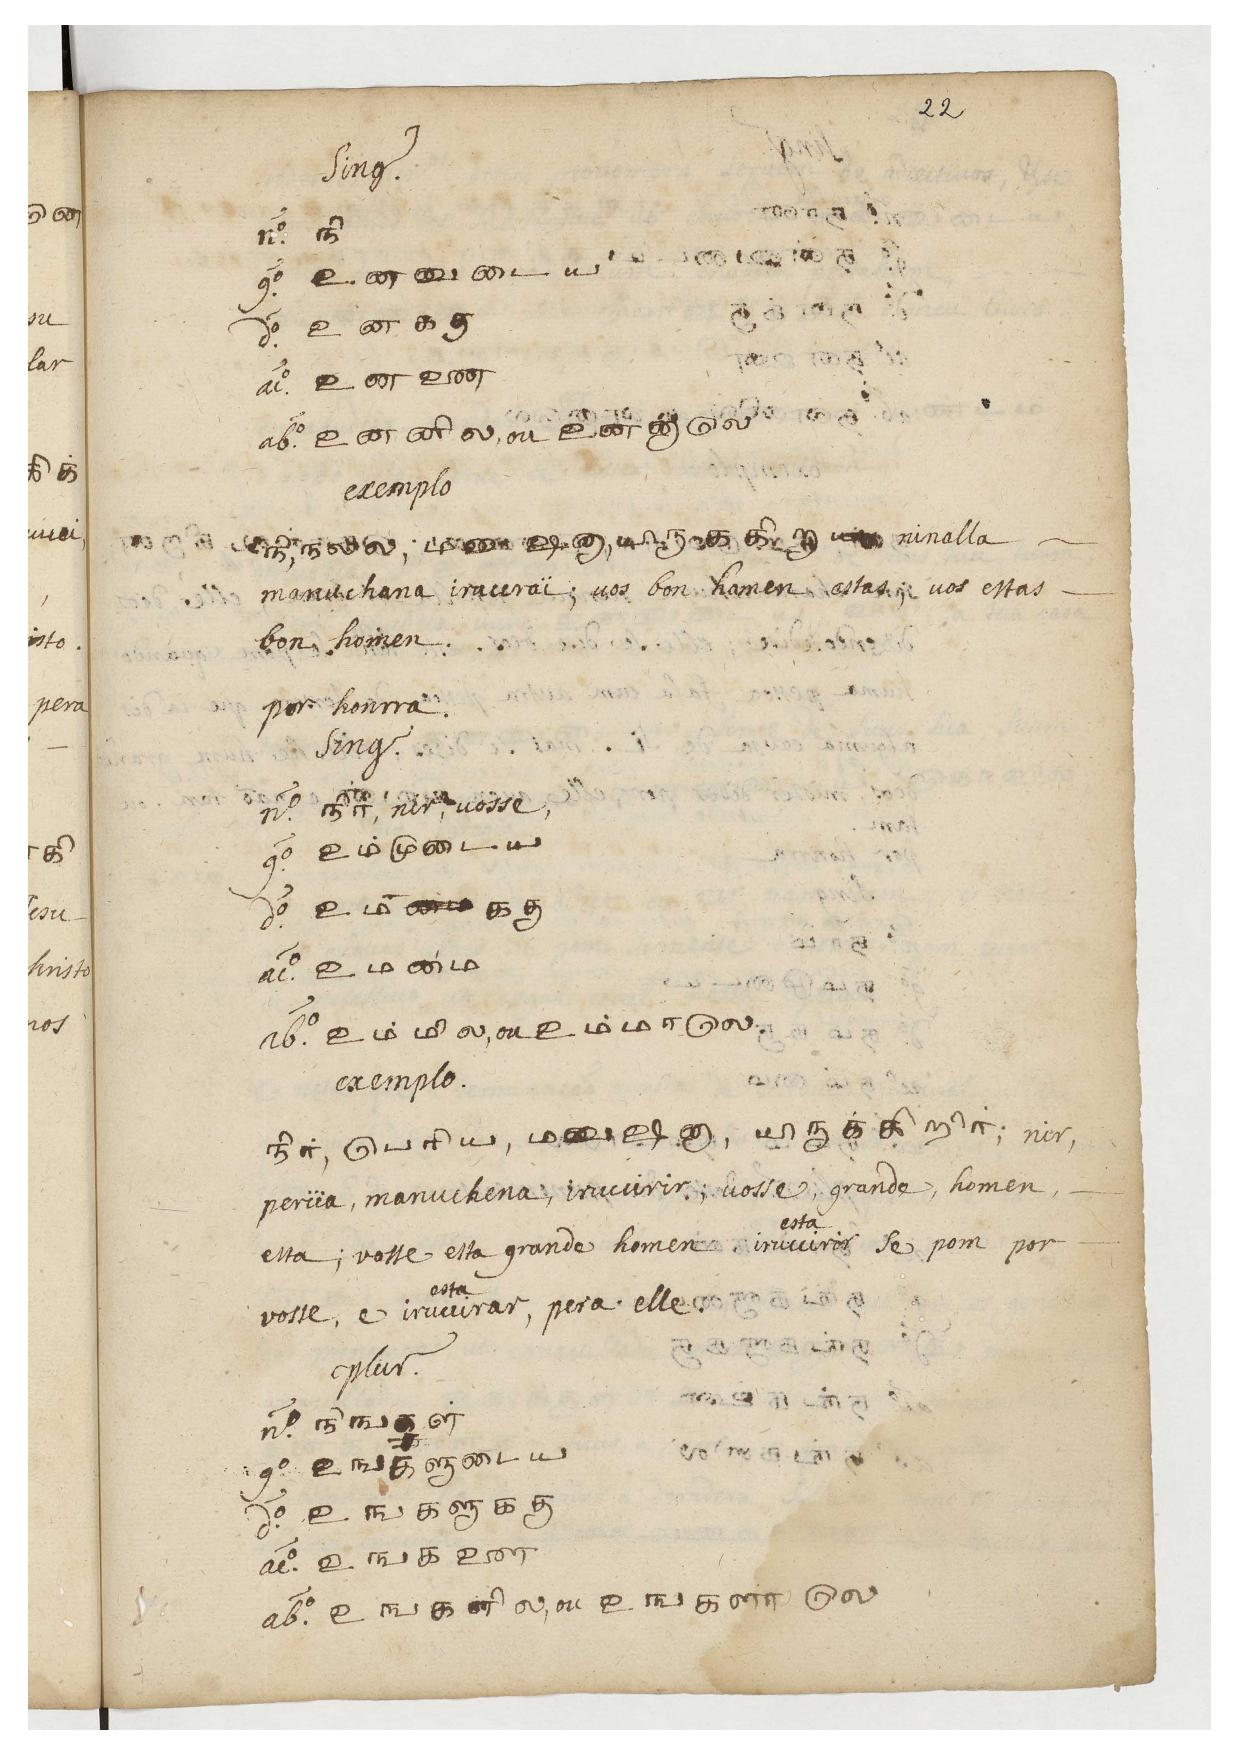
\includegraphics[width=\textwidth]{img-53}}
\newpage
      \chapter*{dos nomes de qualidade e quantitade}
    \addcontentsline{toc}{chapter}{dos nomes de qualidade e quantitade}
    
      

por naõ ter esta lingua nomens proprios da qualidade et quantidade servem pera os 
da qualidade esse participio கொததவன, கொததவள, கொததது, cottaven, cottaval, 
cottadu, pondo lhe antes huma destas particulas அபபடடி, இபபடி, யெபபடி, appadi, 
ippadi, eppadi, அபபடி, ககொததவனானால, யெனககு, வெணடாம, appadi cottavananal 
ïénaccu vendam; si este homen he tal naõ quero della இபபடி, ககொதத, சடடை, உணடாககு, 
ippadi cotta chatti undaccu, faze hum cabay deste modo. 
Cotta segi a mesma regra que nella. 
	
    
  
\@openrighttrue\makeatother
    
\end{document}
    